%%\documentclass[final,3p,times,twocolumn]{elsarticle}
\documentclass[final,3p]{book}

%\includeonly{cs}

%% Use the option review to obtain double line spacing
%% \documentclass[preprint,review,12pt]{elsarticle}

%% Use the options 1p,twocolumn; 3p; 3p,twocolumn; 5p; or 5p,twocolumn
%% for a journal layout:
%% \documentclass[final,1p,times]{elsarticle}
%% \documentclass[final,1p,times,twocolumn]{elsarticle}
%% \documentclass[final,3p,times]{elsarticle}
%% \documentclass[final,3p,times,twocolumn]{elsarticle}
%% \documentclass[final,5p,times]{elsarticle}
%% \documentclass[final,5p,times,twocolumn]{elsarticle}

%% if you use PostScript figures in your article
%% use the graphics package for simple commands
%% \usepackage{graphics}
%% or use the graphicx package for more complicated commands
%% \usepackage{graphicx}
%% or use the epsfig package if you prefer to use the old commands
%% \usepackage{epsfig}

%% The amssymb package provides various useful mathematical symbols
\usepackage{amssymb}
%% The amsthm package provides extended theorem environments
%% \usepackage{amsthm}
%% The bm package lets you access bold symbols in math mode using the \boldsymbol command (useful to get bold greek letters).
\usepackage{bm}
%% The bbm package is contains the indicator function symbol \mathbbm{1}
\usepackage{bbm}
%% The amsmath package contains the split environment, letting you split equations into multiple lines.
%% See "https://www.sharelatex.com/learn/Aligning_equations_with_amsmath " for an explanation.
\usepackage{amsmath}
%% The lineno packages adds line numbers. Start line numbering with
%% \begin{linenumbers}, end it with \end{linenumbers}. Or switch it on
%% for the whole article with \linenumbers after \end{frontmatter}.
%% \usepackage{lineno}
%% The algorithm defines the algorithm floating environment and the algpseudocode package is useful for constructing Pseudo code.
\usepackage{algorithm}
\usepackage{algpseudocode}
%% For creating pictures
\usepackage{tikz}
%% For making algorithms float
\usepackage{float}
\newfloat{algorithm}{t}{lop}
%% For creating draft watermark
%\usepackage{draftwatermark}
%\SetWatermarkText{DRAFT}
%\SetWatermarkScale{1}
\usepackage{pdfpages}

%% Declaring \argmin and \argmax operators:
\DeclareMathOperator*{\argmin}{arg\,min}
\DeclareMathOperator*{\argmax}{arg\,max}
%% Declare trace operator \Tr:
\DeclareMathOperator*{\Tr}{Tr}
%% Declare pdf functions
\DeclareMathOperator*{\Cat}{Cat}
\DeclareMathOperator*{\Dir}{Dir}
\DeclareMathOperator*{\DP}{DP}
\DeclareMathOperator*{\Beta}{Beta}
\DeclareMathOperator*{\GEM}{GEM}
\DeclareMathOperator*{\Stick}{Stick}
\DeclareMathOperator*{\Uniform}{Uniform}
%% shorthand for \boldsymbol and \overline
\let\bs\boldsymbol
\let\ol\overline
%% command that allows equations to be split across pages
%\allowdisplaybreaks[3]

%% natbib.sty is loaded by default. However, natbib options can be
%% provided with \biboptions{...} command. Following options are
%% valid:

%%   round  -  round parentheses are used (default)
%%   square -  square brackets are used   [option]
%%   curly  -  curly braces are used      {option}
%%   angle  -  angle brackets are used    <option>
%%   semicolon  -  multiple citations separated by semi-colon
%%   colon  - same as semicolon, an earlier confusion
%%   comma  -  separated by comma
%%   numbers-  selects numerical citations
%%   super  -  numerical citations as superscripts
%%   sort   -  sorts multiple citations according to order in ref. list
%%   sort&compress   -  like sort, but also compresses numerical citations
%%   compress - compresses without sorting
%%
%% \biboptions{comma,round}

% \biboptions{}


%\journal{MPhil in Scientific Computing}

\begin{document}

%% for elsarticle class
\begin{frontmatter}

%% Title, authors and addresses

%% use the tnoteref command within \title for footnotes;
%% use the tnotetext command for the associated footnote;
%% use the fnref command within \author or \address for footnotes;
%% use the fntext command for the associated footnote;
%% use the corref command within \author for corresponding author footnotes;
%% use the cortext command for the associated footnote;
%% use the ead command for the email address,
%% and the form \ead[url] for the home page:
%%
%% \title{Title\tnoteref{label1}}
%% \tnotetext[label1]{}
%% \author{Name\corref{cor1}\fnref{label2}}
%% \ead{email address}
%% \ead[url]{home page}
%% \fntext[label2]{}
%% \cortext[cor1]{}
%% \address{Address\fnref{label3}}
%% \fntext[label3]{}

\begin{titlepage}
\begin{center}

\includegraphics[width=0.6\textwidth]{Images/cam.png}\\

\vspace*{4cm}
\Huge\textbf{Compressive Sensing in Video Reconstruction}

\vspace*{1.5cm}
\LARGE
\textbf{Brian Azizi}
\vfill

\normalsize
A thesis submitted in partial fulfillment of the requirements for\\
the degree of Master of Philosophy

\vspace{0.8cm}

\normalsize
Supervised by:\\
Dr Anita Faul

\vspace{0.2cm}
Department of Physics\\
Cavendish Laboratory\\
JJ Thomson Avenue\\
CB3 0HE\\
Cambridge, UK\\
\vspace{0.4cm}
\normalsize
\today

\end{center}
\end{titlepage}



\title{Compressive Sensing in Video Reconstruction}

%% use optional labels to link authors explicitly to addresses:
%% \author[label1,label2]{<author name>}
%% \address[label1]{<address>}
%% \address[label2]{<address>}

\author{Brian Azizi}

%\address{Cavendish Laboratory, Department of Physics, J J Thomson
 % Avenue, Cambridge. CB3 0HE}


\tableofcontents

\end{frontmatter}

%%
%% Start line numbering here if you want
%%
% \linenumbers

%% main text
\chapter{Introduction}
The goal of the MPhil project is an implementation of a generic Compressive Sensing algorithm that can efficiently reconstruct video signals from a small number of measurements.

\emph{Compressive Sensing} (CS) \cite{candes2006, donoho2006} is a relatively recent framework within digital signal processing.
Using the techniques in CS, we can measure signals \emph{directly in a compressed format}.

There are two major components to any CS system.
Let $\bm v \in\mathbb{R}^M$ denote the digital signal of interest.
The first component is a \emph{sensing mechanism} that acquires the measurements
\begin{equation}
  \label{eqn:intro_cs}
  \bm\Theta\bm v = \bm y
\end{equation}
where $\bm\Theta$ is a known $N\times M$ matrix with $N<<M$.
The second component is a \emph{reconstruction algorithm} that recovers the original signal $\bm v$ from the CS measurements $\bm y$ by finding a solution to the under-determined system (\ref{eqn:intro_cs}).

In order to solve the system, we make the assumption that $\bm v$ has a sparse representation.
This means that we can perform a change-of-basis transformation
\begin{equation}
  \label{eqn:intro_basis}
  \bm v = \bm\Psi\bm w
\end{equation}
such that the transformed signal $\bm w$ is \emph{sparse}, i.e. it has only a small number of non-zero entries.

Letting $\bm\Phi=\bm\Theta\bm\Psi$, the system (\ref{eqn:intro_cs}) can then be expressed as
\begin{equation}
  \label{eqn:intro_cs2}
  \bm y = \bm\Phi\bm w.
\end{equation}

A variety of deterministic CS algorithms have been developed that attempt to find sparse solutions to (\ref{eqn:intro_cs2}).
For our algorithm, however, we choose to approach the problem from the point of view of \emph{machine learning}.

The aim of supervised machine learning is to learn a relationship $t = f(\bm x)$ between an input vector $\bm x$ and a target $t$.
If the target is a discrete variable the problem is known as \emph{classification}, whereas if $t$ is real-valued we refer to the problem as \emph{regression}.

To apply regression techniques to the CS problem (\ref{eqn:intro_cs2}), we regard the CS measurements $y^{(i)}$ as targets and treat the corresponding rows $\bm\varphi^{(i)}$ of the matrix $\bm\Phi$ is input vectors.
In this context, $\bm y$ is known as a \emph{target vector} and $\bm\Phi$ as the corresponding \emph{design matrix}.
A linear regression algorithm takes these quantities as its input and ``learns'' a \emph{weights vector} $\bm w$.
Given $\bm w$, the original signal can be computed using equation (\ref{eqn:intro_basis}).

For our code, we implemented the \emph{Relevance Vector Machine} (RVM) \cite{tipping2001,tipping2003} as it tends to give very sparse solutions $\bm w$.
This algorithm was used by \cite{pilikos2014} to successfully reconstruct highly undersampled image signals.
Comparing it to a range of classic deterministic CS reconstruction algorithms, \cite{pilikos2014} found that the RVM gave superior reconstruction performance.

In practical CS systems, the sensing mechanism $\bm\Theta$ is typically implemented within the actual sensing hardware.
To provide a range of reconstruction scenarios, our code simulates various types of sensing matrices.

Of particular interest is the case when $\bm\Theta$ corresponds to a signal mask, so that $\bm y$ is a highly undersampled version of the signal $\bm v$.
The problem of solving (\ref{eqn:intro_cs}) is then equivalent to the problem \emph{signal interpolation}.
For this particular class of sensing mechanisms, \cite{pilikos2014} developed an extension to the RVM called \emph{Multi-Scale Cascade of Estimations} (MSCE).
The MSCE algorithm utilizes the multiresolution properties of Haar wavelets to form a cascade of RVMs.
\cite{pilikos2014} investigated its performance in image interpolation and found that it can provide a significant boost in the reconstruction quality.
For our implementation, we extended the MSCE to the case of video interpolation.

\section*{Thesis Organization}
In this thesis, we discuss the underlying theory and implementation details for all the building blocks of our Compressive Sensing algorithm.

We begin in Chapter \ref{ch:cs} with a discussion of the relevant background in digital signal processing.
A brief overview of the conventional approaches to signal acquisition and compression is provided and then contrasted with the novel Compressive Sensing framework.

In order to ensure a high quality reconstruction, it is important to find sparse representations of the signal.
Chapter \ref{ch:dwt} describes the Discrete Cosine Transform and the Discrete Wavelet Transform.
These two basis transforms are often used for their sparsifying properties, especially when applied to digital image and video signals.

In Chapter \ref{ch:rvm}, we derive the Sparse Bayesian Learning framework and discuss two different algorithms for training the RVM.

Chapter \ref{ch:msce} combines Compressive Sensing with Sparse Bayesian Learning to form the Bayesian Compressive Sensing framework.
We show how CS can be viewed from a Bayesian perspective and discuss the MSCE algorith.

Our methods for handling video input are described in Chapter \ref{ch:video} and we provide further implementation details practical considerations in Chapter \ref{ch:code}.

Chapter \ref{ch:results} contains a range of example results as well as a performance evaluation of the code.
Finally, we discuss future work and conclude in Chapter \ref{ch:conclusion}.



\chapter{Background}
\label{ch:cs}
In this chapter, we will introduce the theory of \emph{Compressive Sensing} (also known as \emph{Compressed Sensing, Compressive Sampling} or simply, \emph{CS}).
CS is a framework within signal processing that allows for acquiring signals (i.e. measure or \emph{sense}) directly in a \emph{compressed} format.

To motivate the discussion, we will first review the conventional approach to signal acquisition and compression.

\section{Coventional Signal Processing}
\subsection{Signal Acquisition}
In order to work with information within analog signals (continuous streams of data) such as sounds, images or video, we rely on reducing the analog signals to digital (discrete) signals that can be processed with computers.
This digitization is done by taking discrete measurements of the analog signal at certain points in time or space, a process known as \emph{sampling}.

Conventional approaches to sampling are based on the \emph{Shannon/Nyquist Sampling Theorem} \cite{shannon1949}:
When sampling a signal uniformly, we are able to \emph{perfectly reconstruct} the signal from its samples if the sampling rate is at least twice the highest frequency present in the signal.

Consider an analog signal $x(t)$ that varies with time, such as an audio wave.
Let $f$ be the highest frequency present in $x(t)$.

In order to digitise $x(t)$, we measure $x$ at discrete points in time $t^{(0)}, \cdots, t^{(n)}$ and store the samples $x^{(i)} \equiv x(t^{(i)})$.
We sample $x$ uniformly, measuring a sample every $T_s$ seconds, so that $t^{(i)} = iT_s$.
The sampling rate is therefore $f_s = 1/T_s$.

\begin{figure}
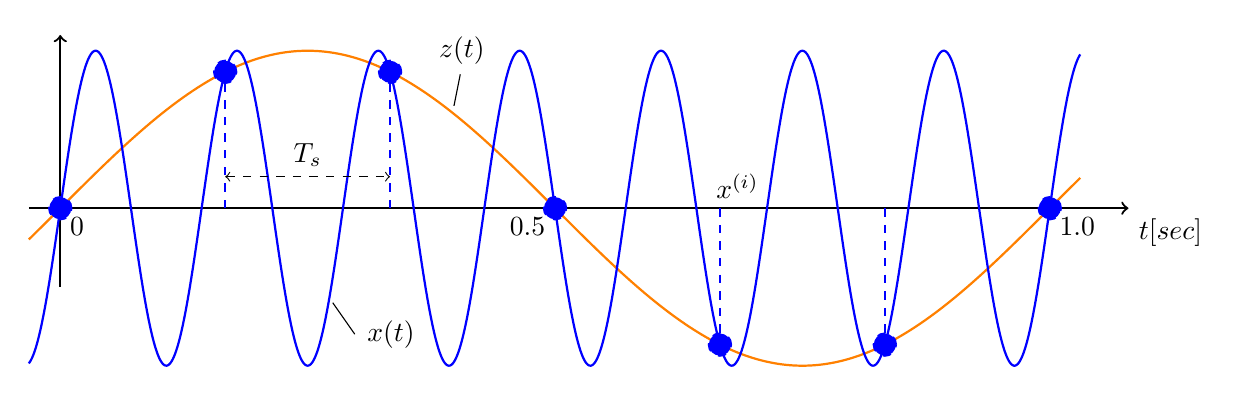
\begin{tikzpicture}[scale=2]
  \draw [thick,->](-0.2,0) -- (2*pi+0.5,0) node[below right] {$t [sec]$};
  \draw [thick,->](0,-0.5) -- (0,1.1);
  \draw [domain=-0.2:2*pi+0.2,samples=1000,orange, thick] plot(\x,{sin(\x r)});
  \draw [domain=-0.2:2*pi+0.2,samples=1000,blue, thick] plot(\x,{sin(7*\x r)});  
  \draw [domain=0:2*pi, samples=7, ycomb, mark=*,blue, dashed, thick] plot(\x,{sin(\x r)});
  \node at (2.55,1) {$z(t)$};
  \draw (2.54,0.85) -- (2.5,0.65);
  \node at (2.1,-0.8) {$x(t)$};
  \draw (1.87,-0.8) -- (1.73,-0.6);
  \node at (4.3,0) [above] {$x^{(i)}$};
  \node at (2*pi,0) [below right] {$1.0$};
  \node at (pi,0) [below left] {$0.5$};
  \node at (0,0) [below right] {$0$};
  \draw [<->, thin, dashed] (pi/3,0.2) -- (pi/2,0.2) node[above] {$T_s$} --(2*pi/3,0.2);
\end{tikzpicture}
\caption[Illustration of Nyquist Sampling]{Illustration of the Shannon/Nyquist Sampling Theorem. The blue curve is the original signal $x(t)$ which is a sinusoid with frequency $f = 7$ Hz. The blue points are discrete samples $x^{(i)}$ taken from $x(t)$ at a sampling rate $f_s = 7$ Hz, which is below the Nyquist Rate $2f = 14$ Hz. Thus, aliasing occurs and interpolation algorithms will reconstruct an alias $z(t)$ (orange curve) of $x(t)$.}
\label{fig:nyquist}
\end{figure}

Suppose we wish to reconstruct $x(t)$ by interpolating the samples.
There is an infinite number of continuous functions that fit this set of samples.
However, it can be shown that only one of them has a bandwidth of no more than $f_s/2$.
Thus, if $f < f_s/2$ (the \emph{Nyquist Criterion}), then $x(t)$ is the unique function that will be approximated by interpolation algorithms such as the \emph{Whittaker-Shannon interpolation formula} \cite{shannon1949}.

In Figure \ref{fig:nyquist}, we have a sinusoidal signal $x(t)$ with frequency $f$.
The sampling rate is $f_s=f$ and therefore below the signal's \emph{Nyquist rate} $2f$. 
Thus, we are unable to reconstruct $x(t)$ from the samples. 
Instead, we will reconstruct an \emph{alias} $z(t)$ which, in this case, is another sinusoid with frequency $f/7$.
The original signal $x$ is lost.

We have illustrated Nyquist sampling in the 1-dimensional case.
The same principles hold for higher dimensional signals such as images and videos.

For signals that vary with space, the sampling rate is governed by the desired spatial resolution.
In order to recover the finer details (the high-frequency components) of an image, we require a higher pixel density (i.e. a larger number of pixels per centimeter (ppcm)).

Nyquist sampling underlies almost all signal acquisition protocols that are found in practice. 
It is the basis of medical imaging, audio and video recording and radio receivers.

\subsection{Signal Compression}
\label{sect:compression}
The sampling theorem imposes a lower bound on the sampling rate above which we are able to perfectly reconstruct the desired signal.
This lower bound is often very high and we end up with a very large number of measurements.
Storage and transfer of such signals becomes prohibitively expensive as the size of the signal grows.
Thus, a need for \emph{data compression} arises.

We will discuss a particular type compression algorithm known as \emph{transform coding}.
It is the standard compression method for a wide range of manmade signals such as audio, photos, and video and is the basis of many common signal formats such as JPEG (images), MPEG (video) and MP3 (audio).

Let $\bm v$ by a real-valued digital signal of length $M$, $\bm v \in \mathbb{R}^M$.
Without loss of generality, $\bm v$ is assumed to be a one-dimensional signal.
If we are working with a multi-dimensional signal, we may first vectorize it into a long vector.
When compressing digital signals, we are usually interested in \emph{lossy compression}.

Any vector in $\mathbb{R}^M$ can be expressed as a linear combination of $M$ \emph{basis vectors} $\bm\psi_j \in \mathbb{R}^M$:
\begin{equation}
\label{eqn:cs-transform1}
  \bm v = \sum_{j=1}^M w_j \bm\psi_j
\end{equation}
where $w_j$ is the coefficient (or weight) associated with $\bm\psi_j$.

By forming the \emph{basis matrix} $\bm\Psi = \left[\bm\psi_1 \,\cdots\, \bm\psi_M\right]$, we can express equation (\ref{eqn:cs-transform1}) in matrix form
\begin{equation*}
\bm v = \bm\Psi \bm w
\end{equation*}
where $\bm w = (w_1,\cdots,w_M)^T$.
For simplicity, we assume that the basis $\bm\Psi$ is orthonormal, so that $\bm\Psi\bm\Psi^T = \bm I_M$ and $\bm\psi_i^T\bm\psi_j$ is 1 if $i = j$ and 0 otherwise.
Thus, the coefficient $w_j$ is given by $w_j = \bm v^T\bm\psi_j$.

We now have two equivalent representations of the same signal, $\bm v$ in the original basis and $\bm w$ in the $\bm\Psi$ basis.
Since $\bm\Psi$ is orthogonal, $\bm v$ and $\bm w$ have the same $\ell_2$-norm, $||\bm v||_2 = ||\bm\Psi\bm w||_2 = ||\bm w||_2$.
However, in the original signal, $\bm v$, the energy is typically spread over many of its components.
On the other hand, it is possible to find a basis $\bm\Psi$ such that the energy of the transformed signal, $\bm w$, is concentrated in only a few large components $w_j$ and a large fraction of its entries are very close to zero.

Suppose that we delete the entries $w_j$ that are very small and replace them with zero to obtain $\bm{\hat w}$.
Let $\bm{\hat v} = \bm\Psi\hat{\bm w}$ the approximate signal in the original domain.
Since $\bm{\hat w}$ is very close to $\bm w$, it follows that
\begin{equation*}
  ||\bm{\hat v} - \bm v||_2 = ||\bm\Psi\bm{\hat w} - \bm\Psi\bm w||_2 = ||\bm\Psi (\bm{\hat w} - \bm w)||_2 = ||\bm{\hat w} - \bm w||_2
\end{equation*}
is very small.

\begin{figure}
  \centering
  \begin{subfigure}[b]{0.4\textwidth}
    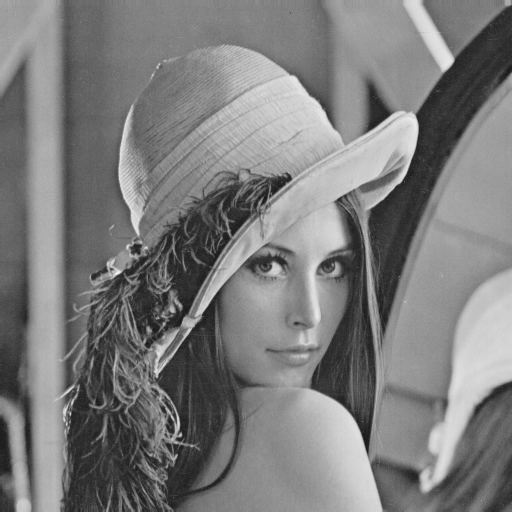
\includegraphics[width=\textwidth]{Chapter2/Images/lenna512.png}
    \caption{Uncompressed Image}
    \label{fig:ch2:lenna_orig}
  \end{subfigure}
  \begin{subfigure}[b]{0.4\textwidth}
    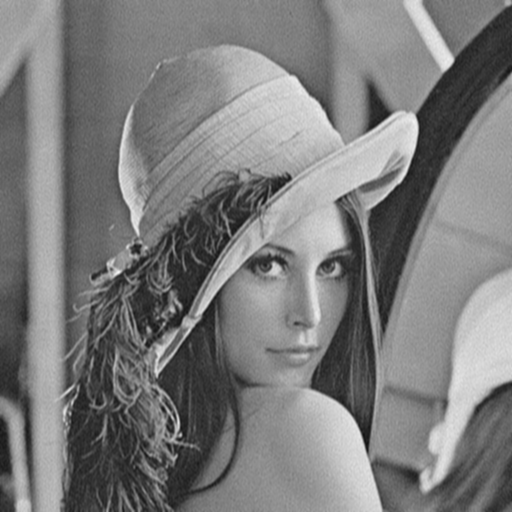
\includegraphics[width=\textwidth]{Chapter2/Images/lenna512_dct.png}
    \caption{Compressed Image via DCT}
    \label{fig:ch2:lenna_dct}
  \end{subfigure}
  \caption[Image Compression using DCT]{The uncompressed image has a resolution of $512\times 512$, i.e. 262,144 pixels. We compress the image by performing a Discrete Cosine Transform (see Section \ref{sect:dct}) and storing only the largest 27,832 coefficients. The compression ratio is 9.42.}
  \label{fig:ch2:dct}
\end{figure}

Thus, a viable method for lossy compression of the signal $\bm v \in \mathbb{R}^M$ would be the following:
\begin{enumerate}
\item Compute the full set of transform coefficients $\{w_j\}_{j=1}^M$ via $\bm w = \bm\Psi^T\bm v$.
\item Locate all the coefficients $w_j$ whose absolute value is above a certain threshold (suppose there are $K$ of them). 
\item Discard all the $(M-K)$ small coefficients
\item Store the values and locations of the $K$ large coefficients
\end{enumerate}
In order to view the compressed signal in the original domain, we reconstruct it via the transform: $\bm\Psi\bm{\hat w} = \bm{\hat v}$, where $\bm{\hat w}$ is $\bm w$ with the $(M-K)$ smallest coefficients replaced by zero.

It is possible to find basis matrices $\bm\Psi$ that result in very high compression ratios for a wide range of signals without any noticable reduction in the signal quality.
Furthermore, many of the commonly used basis transforms can be computed very efficiently.

Audio signals and a wide class of communication signals are highly compressible in the localized Fourier basis.
Images and video signals, on the other hand, can often be compressed via the \emph{Discrete Cosine Transform} (DCT) or the \emph{Discrete Wavelet Transform} (DWT).
For instance, the JPEG standard for image compression is based on the DCT \cite{wallace1992}, while the more modern JPEG2000 format uses the CDF 9/7 wavelet transform or the CDF 5/3 wavelet transform \cite{usevitch2001}.

In Figure \ref{fig:ch2:dct}, we compress the standard test image ``Lenna'' via a DCT. 
We are only storing about 10\% of the transform coefficients.
Yet, the difference between the original image and the compressed image is hardly noticable.

We will discuss the DCT and the DWT in more detail in Chapter \ref{ch:dwt}.

\section{Compressive Sensing}
The conventional approach to data acquisition and compression is very effective and has been highly influential.
However, it is also extremely wasteful.
We acquire a huge amount of data at the signal sampling stage and then proceed to discard a large part of it at the compression stage.

Compressive Sensing \cite{candes2006,donoho2006} is a more general approach that lets us \emph{acquire signals directly in a compressed format}.
This is clearly more efficient as it allows us to skip the intermediate stage of taking $N$ samples.

In this section we will formulate the Compressive Sensing problem.
For simplicity, the focus will be on discrete signals such as digital images or videos.

\subsection{The Compressive Sensing Problem}
Let $\bm v \in\mathbb{R}^M$ be the signal of interest.
As an example, $\bm v$ could be a digital photograph, such as Figure \ref{fig:ch2:lenna_orig}, that has been unrolled into a long vector of length $M$, where $M$ is the number of pixels.

Suppose $\bm v$ is currently unknown and we want to acquire a compressed representation of it without measuring $\bm v$ directly.
To do so, consider the following linear sensing scheme:
We measure inner products between the signal $\bm v$ and a collection of $M$-dimensional vectors $\{\bm\theta_i\}_{i=1}^N$ to obtain the measurements $y_j = \bm v^T\bm\theta_i$ for $i = 1,\cdots,N$. 
This relation can be expressed more succinctly as%Alternatively, we can express equation (\ref{eqn:ch2:sensor1}) as
\begin{equation}
\label{eqn:cs_sensing}
  \bm y = \bm\Theta\bm v
\end{equation}
where $\bm y = (y_1,\cdots,y_N)^T$ and $\bm\Theta$ is the $N\times M$ \emph{sensing matrix} given by
\begin{equation}
\label{eqn:ch2:sensor2}
  \bm\Theta = 
  \begin{bmatrix} 
    \bm \theta_1^T\\
    \vdots\\
    \bm \theta_N^T
  \end{bmatrix}.
\end{equation}

We are interested in the \emph{undersampled} situation where $N < M$.
In particular, we would like to acquire a compressed representation $\bm y$ of $\bm v$ using as few measurements as possible, while still being able to recover the original signal.

There are two problems that stand out at this point. 
\begin{enumerate}
\item Given that $N << M$, how can we ensure that, during the measurement process, we do not lose any information contained in $\bm v$ (i.e. $\bm y$ captures all the information in $\bm v$)?
\item Given our measurements $\bm y$ and knowledge of the sensing matrix $\bm\Theta$, how do we recover the signal of interest $\bm v$?
\end{enumerate}

At an intuitive level, we would expect at least some information to be destroyed during the measurement process, especially if the number of measurements, $N$, is substantially lower than the length of the desired signal, $M$.
Moreover, even if $\bm y$ did contain the same information as $\bm v$, we are still faced with solving the linear system in equation (\ref{eqn:cs_sensing}).
This system is underdetermined and hence there are infinitely many vectors $\bm v$ that satisfy $\bm\Theta\bm v=\bm y$. 

\subsection{Sparse Signals}
In general, we cannot resolve these issues.
However, if we restrict ourselves to a certain class of signals, it is possible to make progress.

In particular, we will focus on signals that have \emph{sparse representations}.
A signal $\bm v \in\mathbb{R}^M$ has a sparse representation if there exists a $M\times M$ basis matrix $\bm\Psi$ so that the transformed signal $\bm w$, where $\bm v = \bm\Psi\bm w$, is \emph{sparse}.

We say that $\bm w$ is \emph{$K$-sparse} if $\bm w$ has $K$ non-zero components.
Equivalently, $\bm w$ is $K$-sparse if 
\footnote{The $\ell_p$-norm of a vector $\bm z \in\mathbb{R}^n$ is defined as follows for $p>0$:
\begin{equation*}
\label{eqn:lp-norm}
  ||\bm z||_p \equiv \left( \sum_{i=1}^n |z_i|^p \right)^\frac{1}{p}.
\end{equation*}
If $p=0$ we can define the $\ell_0$ ``norm'' of $\bm z$ to be the number of its non-zero entries:
\begin{equation*}
\label{eqn:l0-norm}
  ||\bm z||_0 \equiv  \sum_{i=1}^n \mathbbm{1}\{z_j \neq 0\}
\end{equation*}
}
$||\bm w||_0 = K$.

In Section \ref{sect:compression} we noted that many manmade signals are compressible.
They have an almost-sparse representation, meaning that, when expressed in the basis $\bm\Psi$, almost all of their energy is contained in only $K$ components and the remaining components are very close to zero.
Such signals are well-approximated by $K$-sparse representations.

\section{Solving the Compressive Sensing Problem}
So let us suppose then, that the desired signal $\bm v$ is $K$-sparse when expressed in the $\bm\Psi$ basis, where $K$ is 
small ($K << M$).
We can substitute $\bm v = \bm\Psi\bm w$ into (\ref{eqn:cs_sensing}) to get
\begin{equation*}
  \bm y = \bm\Theta\bm v = \bm\Theta\bm\Psi\bm w
\end{equation*}

Let us define $\bm\Phi = \bm\Theta\bm\Psi$, so that
\begin{equation}
  \label{eqn:cs}
  \bm y = \bm\Phi\bm w .
\end{equation}
We have arrived at another underdetermined linear system.
The CS measurements $\bm y$ are still the same as in (\ref{eqn:cs_sensing}), but the sensing matrix $\bm\Theta$ has been replaced by the new sensing matrix $\bm\Phi$.

However, we now want to recover the signal $\bm w$ and we can use the fact that $\bm w$ is $K$-sparse for some $K$.
This allows us to address the problems above.

The information in $\bm w$ is highly localized.
It is fully contained in only $K << M$ of its entries.
Thus, as long as $N\geq K$, it should, at least in principle, be possible for a measurement vector $\bm y$ of length $N<<M$ to completely capture the information within $\bm w$.

Furthermore, since $(M-K)$ entries of $\bm w$ are zero, it follows that in (\ref{eqn:cs}), $\bm y$ is actually linear combination of only $K$ columns of $\bm\Phi$. 
So, if $N\geq K$, we might expect to find suitable constraints that allow us to recover $\bm w$.
Once $\bm w$ is recovered, we can compute $\bm v$ via $\bm v = \bm\Psi\bm w$.

\subsection{Constructing the Sensing Mechanism}
\label{sect:sensors}
In practice, we do not know the locations of the $K$ nonzero entries in $\bm w$.
So the first challenge in a compressive sensing system is to design a $N\times M$ sensing matrix $\bm\Theta$ which ensures that, for any signal $\bm v$ that has a $K$-sparse representation in the basis $\bm\Psi$, we measure all the essential information in the signal.

We will not go into the theoretical details of designing an optimal CS measurement process. Instead we will refer the reader to \cite{candes2008} and simply state three particular sensing matrices that have been used successfully in practice:
\begin{enumerate}
\item Form $\bm\Theta$ by sampling its entries $\theta_{ij}$ independently from the Gaussian distribution with mean zero and variance $1/M$: $\theta_{ij}\, \stackrel{iid}{\sim}\, \mathcal{N}(0,1/M)$.
\item Sample the entries $\theta_{ij}$ independently from a symmetric Bernoulli distribution, $P(\theta_{ij} = \pm 1/\sqrt{M}) = 1/2$. 
\item Form $\bm\Theta$ by starting with the $M\times M$ identity matrix $I_M$ and deleting $M-N$ of its rows at random. This sensing matrix corresponds to measuring a down-sampled version of the signal $\bm v$ directly. If the signal of interest $\bm v$ is a digital image, then $\bm\Theta$ measures $\bm v$ after an \emph{image mask} has been applied to it. This sensing mechanism has been succesfully used in \cite{pilikos2014}.
\end{enumerate}

\subsection{Signal Recovery}
Using the sensing mechanisms outlined above, we are able to measure the signal $\bm v$ directly in a compressed format $\bm y$.
The final part of a Compressive Sensing system is a signal reconstruction algorithm that decompresses $\bm y$ and recovers $\bm v$ or, equivalently, its sparse representation $\bm w$.

This can be achieved by searching for the sparsest solution $\bm w$ that satisfies equation (\ref{eqn:cs}) \cite{baraniuk2007}.
That is, the desired signal is the solution to the optimization problem:
\begin{equation}
\label{eqn:cs_l0}
  \min_{\bm w} ||\bm w||_0 \qquad \mbox{subject to} \qquad \bm\Phi\bm w = \bm y
\end{equation}
Unfortunately, (\ref{eqn:cs_l0}) is an NP-complete problem that can only be solved by an exhaustive search through all possible combinations for the locations of the non-zero entries in $\bm w$.

Luckily, and somewhat surprisingly, it can be shown that, if $N = O(K\log(M/K))$, it is possible to reconstruct $K$-sparse signals exactly by solving the $\ell_1$-optimization problem \cite{baraniuk2007,candes2008}
\begin{equation}
\label{eqn:cs_l1}
  \min_{\bm w} ||\bm w||_1 \qquad \mbox{subject to} \qquad \bm\Phi\bm w = \bm y
\end{equation}
The solution $\bm{\hat w}$ can be transformed to the original domain via $\bm{\hat v} = \Psi\bm{\hat w}$.

In practice, signals $\bm v$ usually only have an almost-sparse representation.
Thus, the reconstruction is not completely exact and the solution $\bm{\hat v}$ will be a close approximation to $\bm v$.

A large part of the CS literature is focused on developing algorithms that recover a signal $\bm v$ from a set CS measurement $\bm y$, either by solving (\ref{eqn:cs_l1}) or through some alternative route.

For a discussion and comparison of some of the most widely used algorithms, see \cite{pilikos2014}.

In Chapter \ref{ch:msce} we will approach the CS signal reconstruction problem in a Bayesian way.
Before we do so, however, we need to introduce the Sparse Bayesian Learning framework (Chapter \ref{ch:rvm}) and provide a more thorough discussion about basis functions (Chapter \ref{ch:dwt}).



\chapter{Basis Functions}
\label{ch:dwt}

%\item Explain MSE, PSNR
In Section \ref{sect:compression}, we introduced transform coding.
We said that any discrete signal $\bm v \in \mathbb{R}^M$ can be expressed in a different basis via a basis transform:
\begin{equation*}
  \bm v = \bm\Psi\bm w
\end{equation*}
where $\bm\Psi$ is the $M\times M$ basis matrix and $\bm w \mathbb{R}^M$ is the representation of $\bm v$ in the $\bm\Psi$ basis.

The particular classes of signals $\bm v$ that we are interested in are digital images and digital video.
The aim of this chapter is to construct a basis matrix $\bm\Psi$ that gives us a (near-) sparse representation of a wide range of such signals $\bm v$.
Finding a set of basis functions $\bs\Psi$ that achieve such a transformation lies at the heart of many lossy compression techniques.

It is important to note here that the choice of basis functions $\bs \Psi$ typically has a significant effect on the performance of the reconstruction algorithms.

\section{Discrete Cosine Transform}
The first basis transform that we will use is the Discrete Cosine Transform (DCT), one of the most widely used transforms in signal processing.
It underlies JPEG image compression and is used in various video compression algorithms such as MJPEG, MPEG, H.261 and H.263 \cite{zeng2013}.
\footnote{A related transform, known as the \emph{Modified DCT} is used in many lossy audio compression formats such as MP3, AAC and Vorbis.}

A DCT decomposes a signal in terms of cosine functions with different frequencies.
Its extensive use in lossy compression algorithms is due to the DCT's \emph{energy compaction} properties.
The majority of a signal's energy is contained within relatively few coefficients - typically those corresponding to the lower frequency basis functions.

On a side note, the DCT comes in a various versions that have minor differences between them.
In the following, we will describe the most widely used version, known as the \emph{DCT-II}, as well as its inverse transform, the \emph{DCT-III}.
We will refer to them simply as ``the DCT'' and ``the Inverse DCT (IDCT)'', respectively.

\subsection{One-Dimensional DCT}
\begin{figure}
  \centering
  \begin{subfigure}{0.45\textwidth}
    \centering
    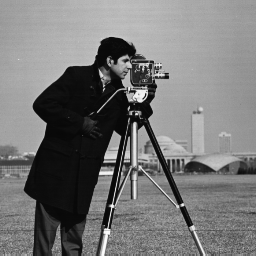
\includegraphics[width=\textwidth]{Chapter3/Images/cameraman.png}
    \caption{Original signal $\bm v$}
  \end{subfigure}
  \begin{subfigure}{0.45\textwidth}
    \centering
    
\includegraphics[width=\textwidth]{Chapter3/Images/dctCoeff.png}
    \caption{DCT of $\bm v$}
  \end{subfigure}
  \caption{Panel (a) shows the original signal $\bm v$, a 256$\times$256 grayscale image known as ``cameraman''. Panel (b) illustrates the 2-D DCT of $\bm v$. The brightness of a an element increases with the absolute value of the corresponding DCT coefficient. (The high-frequency coefficients have been enhanced to show more detail).}
  \label{fig:ch3:dct}
\end{figure}

Formally, the DCT $\bm w$ of a one-dimensional signal $\bm v$ of length $M$ is given by
\begin{equation}
  w_k = c(k) \sum_{m=1}^{M} v_m \, \cos\left(\frac{\pi(2i-1)(k-1)}{2M}\right) \qquad k = 1,\cdots,M
\end{equation}
where
\begin{equation*}
  c(k) = \left\{\begin{array}{ll}
  \sqrt{\frac{1}{M}} & \qquad\mbox{if $k=1$}\\
  \sqrt{\frac{2}{M}} & \qquad\mbox{otherwise}\\
  \end{array}\right.
\end{equation*}
This transforms a signal $\bm v$ in the original domain (time or space) into its representation $\bm w$ in the DCT domain.

\begin{figure}
  \centering
  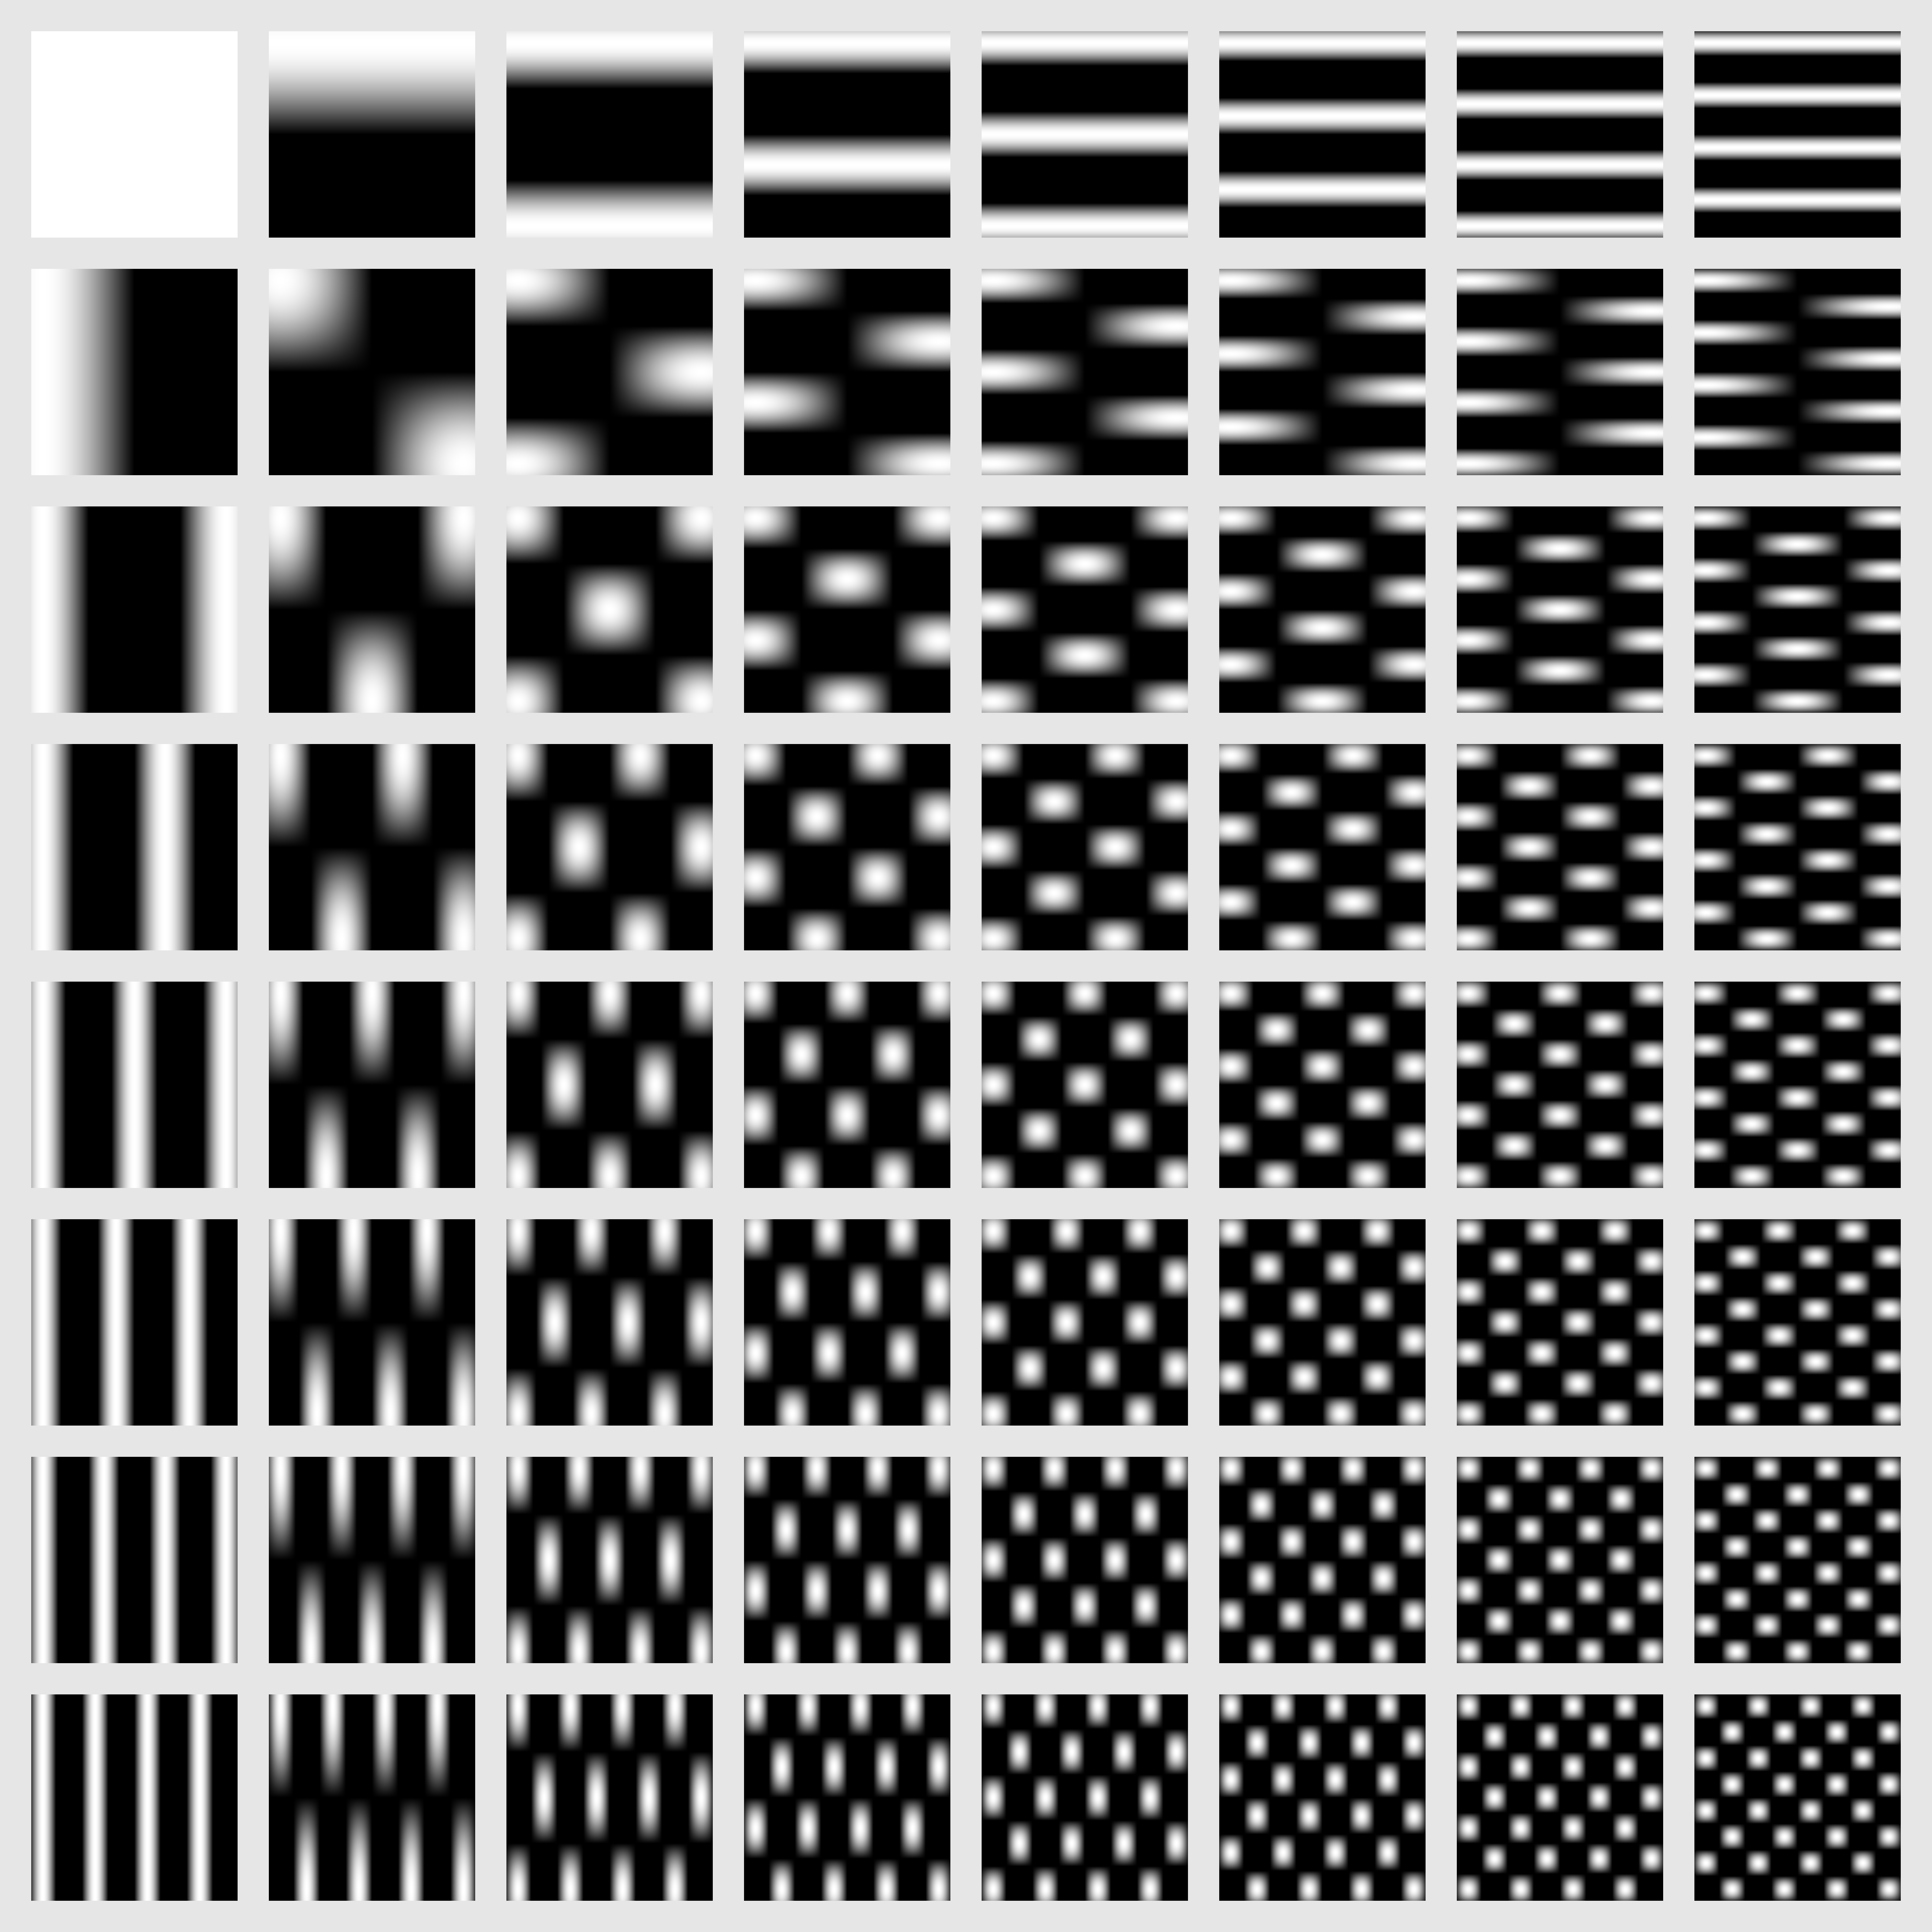
\includegraphics[width=0.5\textwidth]{Chapter3/Images/dct2functions.png}
  \caption{The 2-D DCT basis functions that are used by the DCT to decompose a $8\times 8$ image. 
    The spatial frequency increases towards the bottom right corner.}
  \label{fig:2D-DCT}
\end{figure}

Conversely, given a signal $\bm w$ in the DCT domain, we can transform it back to the orignal (time or space) domain via the IDCT defined by
\begin{equation}
  \label{eqn:idct}
  v_n = \sum_{k=1}^M c(k) w_k  \, \cos\left(\frac{\pi(2i-1)(k-1)}{2M}\right) \qquad n = 1,\cdots,M
\end{equation}

We can express equation (\ref{eqn:idct}) in the desired form $\bm v=\bm P\bm w$.
The entries of the basis matrix $\bm P$ are given by
\begin{equation}
  P_{n,k} = c(k)\, \cos\left(\frac{\pi(2i-1)(k-1)}{2M}\right).
\end{equation}
Note that the basis matrix $\bm P$ is orthogonal, $\bm P^T\bm P=\bm I_M$.

\subsection{Multi-Dimensional DCT}
Once we know how to perform the DCT on a one-dimensional signal, we can easily extend the transform to multi-dimensional signals (images, video, etc).
To do so, we simply perform successive 1-D transforms along each dimension of the signal.
This property is known as \emph{seperability}.

Suppose the signal of interest is a digital image.
That means that $\bm v$ is a $M_1\times M_2$ matrix where $M_1\times M_2$ is the resolution of the image.
To transform the signal, we first perform the DCT on every row of the matrix.
Following that, we perform the DCT on every column of the resulting matrix to get the final transformed signal.

Figure \ref{fig:ch3:dct} shows an example of a 2-D signal $\bm v$ and its transform $\bm w$.
Note that the majority of the energy of the transformed signal is concentrated in the top left corner.
Most of the DCT coefficients are zero or very close to zero.

In Figure \ref{fig:2D-DCT}, we show the 2-D basis functions that would used by the DCT to decompose a signal of size $8\times 8$.
Each basis function is characterised by a horizontal and vertical spatial frequency.
Typically, natural images are mostly made up of low-frequency components and the corresponding coefficients are therefore relatively large.
The highest-frequency components are usually only needed to describe very fine details.

The DCT can be used to decompose video signals with 3-D basis functions. 
Besides the spatial frequencies, the 3-D basis functions have an additional temporal frequency component.
To perform the DCT on a video, we could first perform the 2-D DCT on every frame of the video followed by a 1-D DCT across the temporal axis for each pixel.

For a discussion on the properties of the DCT, see \cite{khayam2003}

\section{Discrete Wavelet Transform}
Wavelets have become a very popular tool in signal processing.
Their energy compaction properties are on par and often superior to those of the DCT for a wide range of signal classes.
In 2000, the JPEG committee released a new image coding standard, JPEG2000, that is gradually replacing the original JPEG standard.
The new format moved away from the DCT and uses a Discrete Wavelet Transform (DWT) instead.

[CAVEAT and INTRO]

\subsection{Introduction to Wavelets}
To motivate wavelets, consider again the one-dimensional signal $\bm v$ of length $M$.
Suppose, for simplicity, that $M$ is a power of $2$, $M = 2^q$ say.
We can view the $\bm v$ as a piecewise-constant function $v(x)$ on the half-open interval $[0,1)$, where $v(x) = v_i$ if $x \in [\frac{i-1}{M}, \frac{i}{M})$.

Let $V^j$ denote the vector space containing all piecewise-constant functions $f$ defined on the interval $[0,1)$ that consist of $2^j$ pieces, each of which is constant across a sub-interval of size $2^{-j}$.
Thus, $V^0$ consists of all functions that are constant on $[0,1)$, while $V^1$ consists of all functions that have two constant pieces, one over $[0,1/2)$ and one over $[1/2,1)$.
In particular, our signal $v(x)$ resides in the space $V^q$.

Note that if $f \in V^j$, then $f \in V^{j+1}$.
Thus, the vector spaces $V^j$ are nested: $V^0 \subset V^1 \subset V^2 \subset \cdots$.

Next, we need to choose a basis for each vector space $V^j$.
To do so, we introduce a \emph{scaling function} (also known as \emph{scalet}, or \emph{father wavelet}) that is usually denoted $\phi(x)$.
The form of the scaling function depends on the particular choice wavelet decomposition.

\begin{figure}
  \centering
  \begin{subfigure}{0.4\textwidth}
    \centering
    \begin{tikzpicture}[xscale=2]
      \draw [thin,->] (0,-1.5) -- (0,1.5);
      \draw [thin,->] (-0.5,0) -- (1.5,0) node[below]{\small$x$};
      \draw [very thick] (-0.2,0) -- (0,0) node[below left]{\small$0$} -- (0,1) node[left]{\small$1$} -- (1,1) -- (1,0) node[below]{\small$1$} -- (1.3,0);
    \end{tikzpicture}
    \caption{Haar scaling function $\phi(x)$}
    \label{fig:haar_scaling}
  \end{subfigure}
  \begin{subfigure}{0.4\textwidth}
    \centering
    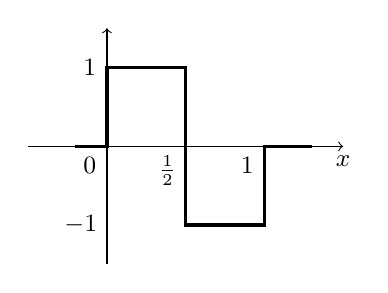
\begin{tikzpicture}[xscale=2]
      \draw [thin,->] (0,-1.5) -- (0,1.5);
      \draw [thin,->] (-0.5,0) -- (1.5,0) node[below]{\small$x$};
      \draw [very thick] (-0.2,0) -- (0,0) node[below left]{\small$0$} -- (0,1) node[left]{\small $1$} -- (0.5,1) -- (0.5,-1) -- (1,-1) -- (1,0) node[below left]{\small $1$} -- (1.3,0);
      \node at (0,-1)[left]{\small$-1$};
      \node at (0.5,0)[below left]{\small $\frac{1}{2}$};
    \end{tikzpicture}
    \caption{Haar mother wavelet $\psi(x)$}
    \label{fig:haar_mother}
  \end{subfigure}
  \caption{The scaling function and wavelet function for the Haar wavelets.}
  \label{fig:haar_1d}
\end{figure}

For example, for the \emph{Haar wavelets} the scaling function is given by
\begin{equation}
  \label{eqn:haar_scale}
  \phi(x) = \left\{ \begin{array}{rl}
    1& \qquad \mbox{if $0\leq x < 1$}\\
    0& \qquad \mbox{otherwise}
  \end{array}\right.
\end{equation}
See Figure \ref{fig:haar_scaling} for a plot of $\phi(x)$.

Given the scaling function $\phi(x)$, we can define the following basis for $V^j$:
\begin{equation*}
  \phi_k^j(x) := 2^{j/2}\phi(2^j x-k) \qquad k = 0,\cdots, 2^j-1
\end{equation*}

Using this basis, we can decompose our signal $v(x)\in V^q$ as 
\begin{equation*}
  v(x) = \sum_{k=0}^{2^q-1} c_k^q \phi_k^q(x)
\end{equation*}
For the scaling function defined in equation (\ref{eqn:haar_scale}), we have that $c_k^q = v_{k+1}$.

To obtain \emph{wavelets}, consider the \emph{orthogonal complement} of $V^j$ in $V^{j+1}$ and denote it $W^j$. 
That is, $W^j = \{f \in V^{j+1} :\quad \langle f,g\rangle = 0\quad \forall g \in V^j\}$ where the inner product $\langle f,g\rangle$ is given by
\begin{equation*}
  \langle f,g\rangle = \int_0^1f(x)g(x)dx.
\end{equation*}
By forming a basis for $W^j$, we obtain a set of \emph{wavelet functions} $\{\psi_k^j,\, k=0,\cdots,2^j-1\}$.
Wavelet functions can be constructed by scaling and shifting a so-called \emph{mother wavelet} $\psi(x)$ as follows:
\begin{equation*}
  \psi_k^j(x) = 2^{j/2}\psi(2^j x - k) \qquad k = 0,\cdots, 2^j-1
\end{equation*}

For the Haar wavelets, the mother wavelet is given by:
\begin{equation*}
  \psi(x) = \left\{\begin{array}{rl}
  1&\qquad 0 \leq x < 1/2\\
  -1&\qquad 1/2 \leq x < 1\\
  0&\qquad\mbox{otherwise}
  \end{array}\right.
\end{equation*}
The Haar mother wavelet is shown in Figure \ref{fig:haar_mother}.

Note that, since the scaling functions $\phi_k^j$ form a basis of $V^j$ and the wavelet functions $\psi_k^j$ form a basis of $W^k$, and since $W^j$ is the orthogonal complement to $V^j$ in $V^{j+1}$, it follows that the set $\{\phi_k^j, \psi_k^j: k=0,\cdots,2^j-1\}$ forms a basis of the vector space $V^{j+1}$.

This allows us to express our signal $v \in V^q$ as 
\begin{equation*}
  v(x) = \sum_{k=0}^{2^{q-1}-1} d_k^{q-1}\psi_k^{q-1}(x) + \sum_{k=0}^{2^{q-1}-1} c_k^{q-1}\phi_k^{q-1}(x)
\end{equation*}
This gives us the first level of the discrete wavelet transform of $v$.
The coefficients $c_k$ and $d_k$ are sometimes referred to as ``approximation'' coefficients and ``detail'' coefficients, respectively.

We can continue the decomposition by splitting the basis for $V^{q-1}$ into the bases for $V^{q-2}$ and $W^{q-2}$ to get the next level of the transform:
\begin{equation*}
  v(x) = \sum_{k=0}^{2^{q-1}-1} d_k^{q-1}\psi_k^{q-1}(x) + \sum_{k=0}^{2^{q-2}-1} d_k^{q-2}\psi_k^{q-2}(x) + \sum_{k=0}^{2^{q-2}-1} c_k^{q-2}\phi_k^{q-2}(x)
\end{equation*}
To get the full decomposition, we continue in this fashion up to the $q$th level:
\begin{equation*}
  v(x) = \sum_{j=0}^{q-1} \sum_{k=0}^{2^j-1} d_k^{j} \psi_k^j(x) + c_0^0\phi(x)
\end{equation*}
The full DWT of $\bm v$ consists of the coefficients $\{c_0^0, d_k^j:\,j=0,\cdots,q-1, \, k=0,\cdots,2^j-1\}$.


\subsection{Computing the DWT}

\begin{figure}
  \centering
  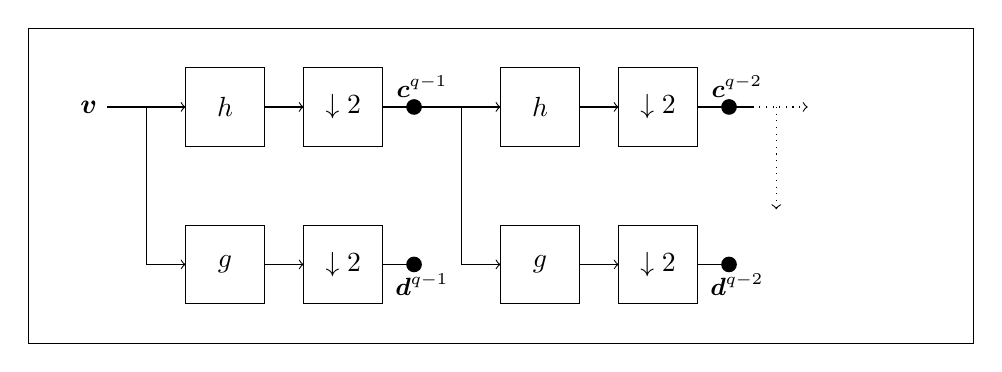
\begin{tikzpicture}
    \draw (0,0) rectangle (12,4);
    \draw (1,3) node[left]{$\bm v$} -- (1.5,3);
    \draw (1.5,1) -- (1.5,3);
    \draw [->](1.5,3) -- (2,3);
    \draw [->](1.5,1) -- (2,1);
    \draw (2,2.5) rectangle (3,3.5);
    \node at (2.5,3) {$h$};
    \draw (2,0.5) rectangle (3,1.5);
    \node at (2.5,1) {$g$};
    \draw [->](3,1) -- (3.5,1);
    \draw (3.5,0.5) rectangle (4.5,1.5);
    \node at (4,1) {$\downarrow 2$};
    \draw (4.5,1) -- (5,1) node [below] {\small$\bm d^{q-1}$};
    \node at (4.9,1)[shape=circle, fill=black, inner sep=2pt, minimum size=2pt] {};
    \draw [->](3,3) -- (3.5,3);
    \draw (3.5,2.5) rectangle (4.5,3.5);
    \node at (4,3) {$\downarrow 2$};
    \draw [->](4.5,3) -- (6,3);
    \draw [->](5.5,3) -- (5.5,1) -- (6,1);
    \node at (5,3) [above] {\small$\bm c^{q-1}$};
    \node at (4.9,3) [shape=circle, fill=black, inner sep=2pt, minimum size=2pt] {};
    \draw (6,2.5) rectangle (7,3.5);
    \node at (6.5,3){$h$};
    \draw (6,0.5) rectangle (7,1.5);    
    \node at (6.5,1){$g$};
    \draw [->] (7,3) -- (7.5,3);
    \draw (7.5,2.5) rectangle (8.5,3.5);
    \node at (8,3) {$\downarrow 2$};
    \draw [->] (7,1) -- (7.5,1);
    \draw (7.5,0.5) rectangle (8.5,1.5);
    \node at (8,1) {$\downarrow 2$};
    \draw (8.5,1) -- (9,1) node [below] {\small$\bm d^{q-2}$};
    \node at (8.9,1) [shape=circle, fill=black, inner sep=2pt, minimum size=2pt] {};
    \draw (8.5,3) -- (9.2,3);
    \draw [->,dotted](9.2,3) -- (9.9,3);
    \draw [->,dotted](9.5,3) -- (9.5,1.7);
    \node at (8.9,3) [shape=circle, fill=black, inner sep=2pt, minimum size=2pt] {};
    \node at (9,3) [above] {\small$\bm c^{q-2}$};
  \end{tikzpicture}
  \caption{The first two levels of the DWT of the signal $\bm v$ of length $2^q$ via a filter bank.}
  \label{fig:filterbank}
\end{figure}

In practice, we can compute one level of the DWT coefficients by passing the signal $\bm v$ through a \emph{low-pass filter} $\bm h$ and a high-pass filter $\bm g$, respectively, and then downsampling the results by a factor of two.
Overall, these computations can be done by multiplying the vector $\bm v$ by a matrix $\bm H$ and a matrix $\bm G$ to get the approximation and detail coefficients, repectively.

To compute the next level, we take the approximation coefficients of the current stage and pass them again through the filter bank.
The procedure is depicted in Figure \ref{fig:filterbank}.




%% The simplest wavelet basis transformation is based on the Haar wavelets.
%% Figure \ref{fig:haarlenna} vizualises a basis transformation of the original image $\bs x$ to $\bs w$. 
%% This example uses a Haar wavelet basis at the first scale.
%% We will explain the Haar wavelet transformations of images and videos in more detail in the next chapter.
%% Dark areas correspond to small coefficients.
%% Note that most entries in $\bs w$ are near zero. 
%% In practice, we approximate these entries as zero and treat $\bs w$ as sparse.

%% \begin{figure}
%% \center
%% 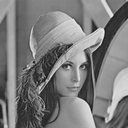
\includegraphics{Images/128.png}
%% 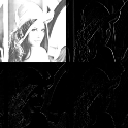
\includegraphics{Images/haar.png}
%% \caption{Original image $\bs x$ (left) and its Haar basis transformation $\bs w$ (right). See next chapter for more details on Haar wavelets.}
%% \label{fig:haarlenna}
%% \end{figure}

%% \section{Haar basis functions}
%% The RVM takes as input a target vector ($\bs y$) and a basis matrix ($\bs \Psi$). 
%% In this respect, it is agnostic about whether the signal is an image or video or of some other type alltogether.
%% Most of this information is encoded in the basis matrix $\bs \Psi$.
%% It is therefore important, and often challenging, to select a good set of basis functions.

%% Our current implementation uses 3-dimensional Haar wavelet basis functions.
%% I will show how the basis matrix $\bs\Psi$ is constructed by briefly describing how the discrete Haar wavelet transform is performed on 1D, 2D and finally on 3D signals.
%% \subsection{1D Haar wavelet transform}
%% Consider a 1-dimensional signal $\bs s = \{s_1,\dots,s_r\} \in \mathbb{R}^r$ ($r$ for ``rows''), where, for simplicity, we assume that $r$ is a power of 2.
%% The Haar wavelet transform can be performed at various resolution scales.
%% The transform at the first scale is given by:
%% \begin{equation*}
%% \bs s = \{s_1,\dots,s_r\}\to \frac{1}{\sqrt{2}}\{s_1+s_2,s_3+s_4,\dots,s_{r-1}+s_r,s_1-s_2,\dots,s_{r-1}-s_r\}=\hat{\bs s}^{(1)}
%% \end{equation*}
%% The first half of the signal is replaced by scaled averages of adjacent elements and the second half is replaced by scaled differences of adjacent elements.
%% By performing this transform again on the first half of $\hat{\bs s}^{(1)}$ while keeping the second half fixed, we get the Haar wavelet transform at the second scale $\hat{\bs s}^{(2)}$. 
%% To get the third scale transform $\hat{\bs s}^{(3)}$, we perform the initial transform on the first quarter of $\hat{\bs s}^{(2)}$ while keeping the rest of the signal fixed.
%% We may continue this process until we reach the $i$th scale, where $2^i = r$.

%% From here on, we will only consider the first scale transform $\hat{\bs s}^{(1)}$ and we will omit the $(1)$ superscript.
%% We can express the transform as a multiplication by an orthogonal $r\times r$ matrix $W$ given by
%% \begin{equation}
%% W = \begin{bmatrix}
%%   \Phi_r \\
%%   \Psi_r \\
%% \end{bmatrix}
%% \end{equation}
%% where $\Phi_r$ and $\Psi_r$ are $(r/2)\times r$ matrices\footnote{Note that the matrix $\Psi_r$ used here is different to the matrix $\Psi$ that was used in the previous chapter (which corresponds to $W^T$ here).} given by
%% \begin{equation*}
%% \Phi_r = \frac{1}{\sqrt{2}} \begin{pmatrix}
%% 1&1&0&0&\cdots&0&0\\
%% 0&0&1&1&\cdots&0&0\\
%% \vdots&\vdots&\vdots&\vdots&\ddots&\vdots&\vdots\\
%% 0&0&0&0&\cdots&1&1
%% \end{pmatrix}
%% \end{equation*}
%% and 
%% \begin{equation*}
%% \Psi_r = \frac{1}{\sqrt{2}} \begin{pmatrix}
%% 1&-1&0&0&\cdots&0&0\\
%% 0&0&1&-1&\cdots&0&0\\
%% \vdots&\vdots&\vdots&\vdots&\ddots&\vdots&\vdots\\
%% 0&0&0&0&\cdots&1&-1
%% \end{pmatrix}
%% \end{equation*}


%% In the signal processing literature, $\Phi_r$ is referred to as a low pass filter, while $\Psi_r$ is referred to as a high pass filter.
%% $\Phi_r$ outputs an average of the signal and $\Psi_r$ outputs the details of the signal.

%% \subsection{2D Haar wavelet transform}
%% Let $A \in \mathbb{R}^{r\times c}$ be a 2-dimensional signal (e.g. an image).
%% For simplicity, we will assume that both $r$ and $c$ are powers of 2 (though not necessarily equal).

%% It is simple to obtain $A$'s Haar wavelet transform $\hat{A}$ at the first scale.
%% This is done by first applying the 1-dimensional transform individually to each column of $A$ to obtain a temporary matrix $\hat A_{temp}$.
%% Next, we apply the 1-dimensional haar wavelet transform individually to each row of $\hat A_{temp}$ to obtain $\hat A$.

%% We can again express the transform as a multiplication of matrices:
%% \begin{equation}
%% \label{eqn:2Dtransform}
%% \hat A = \begin{bmatrix}
%%   \Phi_r\\
%%   \Psi_r\\
%% \end{bmatrix}
%% A
%% \begin{bmatrix}
%%   \Phi_c^T & \Psi_c^T\\
%% \end{bmatrix}
%% \end{equation}
%% where $\Phi_r$ and $\Psi_r$ are as before and $\Phi_c$ and $\Psi_c$ are of similar form but each have dimensions $(c/2)\times c$.
%% This is the transform that was used to generate the RHS of Figure \ref{fig:haarlenna}.
%% We note that the high-pass filters essentially detect edges of various orientations in the image.

%% However, as it currently stands, we cannot use this form of the basis transformation for the reconstruction algorithm. Recall that the RVM requires a \emph{vector} of measurements as opposed to a matrix and also that it requires a single basis matrix, not a basis transform as given in (\ref{eqn:2Dtransform}).

%% To do this, we store the 2-dimensional signal $A$ as a long column vector $\bs a$ of length $rc$ by pasting the individual columns of $A$ one after another.
%% The basis transformation of $\bs a$ can then be expressed as 
%% \begin{equation*}
%% \hat{\bs a} = W \bs a
%% \end{equation*}
%% where $W$ is a $rc \times rc $ matrix given by
%% \begin{equation*}
%% W = 
%% \begin{bmatrix}
%% \Phi_c \otimes \Phi_r \\
%% \Phi_c \otimes \Psi_r \\
%% \Psi_c \otimes \Phi_r \\
%% \Psi_c \otimes \Psi_r \\
%% \end{bmatrix}
%% \end{equation*}

%% The symbol $\otimes$ denotes the \emph{Kronecker product}. 
%% The kronecker product $P \otimes Q$ between matrices $P$ and $Q$ with dimensions $m_P \times n_P$ and $m_Q \times n_Q$, respectively,  is defined to be the block matrix
%% \begin{equation*}
%% \begin{bmatrix}
%% p_{1,1} Q & p_{1,2} Q & \cdots & p_{1,n_P} Q \\
%% p_{2,1} Q & p_{2,2} Q & \cdots & p_{2,n_P} Q \\
%% \vdots&\vdots&\ddots&\vdots \\
%% p_{m_P,1} Q & p_{m_P,2} Q & \cdots & p_{m_P,n_P} Q \\
%% \end{bmatrix}
%% \end{equation*}
%% of size $m_Pm_Q \times n_Pn_Q$.

%% \subsection{3D Haar wavelet transform}
%% Let $V \in \mathbb{R}^{r\times c\times s}$ be a 3-dimensional signal such as a video. 
%% $V$ has $r$ rows, $c$ columns and $s$ slices, and we assume that $r$, $c$ and $s$ are all powers of 2. 
%% We may visualize $V$ as a ``volume'' with 2 spacial dimensions and one time dimension corresponding to frames of the video.

%% To obtain the Haar wavelet transform $\hat V$ of $V$, we first perform the 1-dimensional transform individually on each column in every slice of $V$ to get $\hat V_{temp1}$.
%% We then perform the 1D transform on every row in every slice of $\hat V_{temp_1}$ to get $\hat V_{temp_2}$.
%% Finally, we perform the 1D transform across the slices for every row and column to get $\hat V$.

%% However, like in the 2-dimensional case, we need to be able to pass a single vector of coefficients and a single basis matrix to the RVM.
%% To do this, we vectorize $V$ as follows. 
%% First, we vectorize each individual slice of $V$ as before in the 2D case.
%% Then, we stack all these vectors on top each other to get one very long column vector $\bs v$ of length $rcs$.
%% The Haar wavelet transform is given by 
%% \begin{equation*}
%% \hat{\bs v} = W \bs v
%% \end{equation*}
%% where 
%% \begin{equation*}
%% W = 
%% \begin{bmatrix}
%% \Phi_s \otimes \Phi_c \otimes \Phi_r \\
%% \Phi_s \otimes \Phi_c \otimes \Psi_r \\
%% \Phi_s \otimes \Psi_c \otimes \Phi_r \\
%% \Phi_s \otimes \Psi_c \otimes \Psi_r \\
%% \Psi_s \otimes \Phi_c \otimes \Phi_r \\
%% \Psi_s \otimes \Phi_c \otimes \Psi_r \\
%% \Psi_s \otimes \Psi_c \otimes \Phi_r \\
%% \Psi_s \otimes \Psi_c \otimes \Psi_r \\
%% \end{bmatrix}
%% \end{equation*}


%% \subsection{Daubechies Wavelets}
%% \emph{Intuition. Where do the coeffs come from. Matrices. Boundary conditions.}


%% \section{Forming the basis matrix}
%% \emph{1D, 2D, 3D case. Different scales}

%% For a deeper introduction into wavelets see \cite{stollnitz1995}.
%% For more information on wavelet compression techniques, see \cite{devore1992}.





\include{chapter}

\chapter{Bayesian Compressive Sensing}
\label{ch:msce}

In this chapter, we combine the Compressive Sensing framework from Chapter \ref{ch:cs} with the Sparse Bayesian Learning framework from Chapter \ref{ch:rvm} to formulate the \emph{Bayesian Compressive Sensing} (BCS) algorithm.

Following that, we discuss the scenario where the sensing mechanism $\bm\Theta$ corresponds to a signal mask and describe how the performance of the BCS algorithm can be boosted via the \emph{Multi-Scale Cascade of Estimations} algorithm.

\section{Compressive Sensing as Linear Regression}
In the Bayesian Compressive Sensing (BCS) \cite{ji2008} framework, we approach the Compressive Sensing problem from the point of view of linear regression.

Recall the setup from Chapter \ref{ch:cs}.
We are intersted in recovering the signal $\bm v\in\mathbb{R}^M$ from the CS measurements $\bm\Theta\bm v = \bm y\in\mathbb{R}^N$, where $N << M$.
We also assume that $\bm v$ is compressible in the basis $\bm \Psi$.

This means that $\bm w = \bm\Psi^T\bm v$ is well approximated by the $K$-sparse vector $\bm w_K$ which is identical to $\bm w$ for the $K$ elements in $\bm w$ with the largest magnitude.

Thus, $\bm w_e = \bm w - \bm w_K$ is assumed to be very small in magnitude.
Letting $\bm\Phi=\bm\Theta\bm\Psi$, we have
\begin{equation*}
  \bm y = \bm\Theta\bm v = \bm\Theta\bm\Psi\bm w = \bm\Phi\bm w = \bm\Phi\bm w_K + \bm\Phi\bm w_e = \bm\Phi\bm w_K + \bm n_e
\end{equation*}
where $\bm n_e = \bm\Phi\bm w_e$ will be regarded as noise.
Furthermore, there could be an additional noise source $\bm n$ in the CS measurements $\bm y$ (e.g. due to finite precision in the measurement device) so that, overall,
\begin{equation}
\label{eqn:bcs_setup}
  \bm y = \bm\Phi\bm w_K + \bm n_e + \bm n = \bm\Phi\bm w_K + \bm \epsilon
\end{equation}
with $\bm\epsilon = \bm n_e + \bm n$.

In the BCS literature \cite{ji2008}, $\bm\epsilon$ is typically approximated by a zero-mean Gaussian noise variable with an unknown variance $\sigma^2$:
\begin{equation}
\label{eqn:bcs_noise}
  \bm\epsilon\sim\mathcal{N}(0,\sigma^2\bm I_N).
\end{equation}

Although this assumption may not always be completely accurate in practice, it is often used for its desirable analytical properties.
A possible justification is that the sensing matrix $\bm\Theta$ is usually constructed randomly (often using Gaussian samples) and that the noise source $\bm n$ in the CS measurements is typically represented by a zero-mean Gaussian distribution.

Note the similarity between equations (\ref{eqn:bcs_setup}) and (\ref{eqn:bcs_noise}) and the geneneral linear regression model in equations (\ref{rvm:lklhd_2}) and (\ref{rvm:error}).
The only difference is that, in equation (\ref{eqn:bcs_setup}), we have the addtional constraint that $\bm w_K$ is \emph{sparse}.

Since in the BCS framework, we wish to solve the CS problem from a Bayesian standpoint, we are interested in computing a full posterior distribution of the weights $\bm w_K$ and the noise variance $\sigma^2$.
The sparsity constraint can be entered into the model by placing a sparseness-inducing prior distribution over the weights $\bm w_K$.

There is a range of popular sparseness priors.
However, to make the connection to the RVM and exploit the analysis from Chapter \ref{ch:rvm}, we choose the prior from (\ref{eqn:prior_w}):
\begin{equation*}
  p(\bm w_K\,|\,\bm \alpha) = \prod_{j=1}^M \mathcal{N}\left(w_j\,|\,0,\alpha_j^{-1}\right)
\end{equation*}

To summarize, we solve the CS problem by passing the CS measurements $\bm y$ and the matrix $\bm\Phi$ to train a RVM.
The SBBL algorithm (Algorithm \ref{rvm:alg2}) is then used to compute the posterior distribution of the weights $\bm w \in \mathbb{R}^M$ (\ref{rvm:posterior}).

The desired signal $\bm v\in\mathbb{R}^M$ can then by recovered by computing 
\begin{equation}
  \label{eqn:bcs_recover}
  \bm{\hat v} = \bm\Psi\bm\mu
\end{equation} 
where $\bm \mu$ is the posterior mean of $\bm w$.

The method of applying the RVM to CS inversion is sometimes referred to as the Bayesian Compressive Sensing (BCS) algorithm.
The BCS algorithm was compared against state-of-the-art deterministic CS algorithms by \cite{ji2008,pilikos2014} and shown to give comparable performance.

We have implemented the BCS algorithm as part of our Compressive Sensing algorithm.
Using BCS, our implementation is able to reconstruct video signals from a small number of CS measurements that were sampled by a general sensing mechanism $\bm\Theta$. 


\section{The Case when \texorpdfstring{$\bm\Theta$}{[Theta]} is a Signal Mask}

\subsection{Signal Interpolation}
\begin{figure}
  \centering
  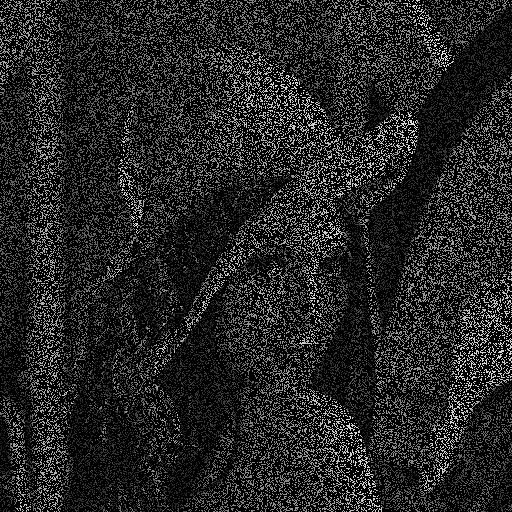
\includegraphics[width=0.6\textwidth]{Chapter5/Images/lenna_MASKED.png}
  \caption[Example of masked image signal]{Example of an image with missing pixel values. The missing data points are set to zero and displayed in black}
  \label{fig:lenna_mask}
\end{figure}

If the sensing matrix $\bm\Theta$ is a signal mask (see Section \ref{sect:sensors}), the CS measurements $y$ of an image $\bm v$ can be visualized as an image with missing pixel values as in Figure \ref{fig:lenna_mask}.
The problem of reconstructing such signals is sometimes referred to as \emph{interpolation}.

In this context, the design matrix $\bm\Phi$ can be computed efficiently from $\bm\Psi$ by simply deleting all the rows in $\bm\Psi$ that correspond to the entries of $\bm v$ that have missing data.

Moreover, we can get a slight performance boost in the reconstruction by filling in the BCS solution $\bm{\hat v}$ (\ref{eqn:bcs_recover}) with the measured at data $\bm y$ at the appropriate locations.

\subsection{Reconstruction using Haar Wavelets}
\label{sect:interpol_haar}
Using the BCS model from above with a Haar basis matrix, we reconstruct the image in Figure \ref{fig:lenna_mask} and display the output in Figure \ref{fig:lenna_rvm} for various scales of the Haar basis.
\begin{figure}
\centering
  \begin{subfigure}{0.4\textwidth}
    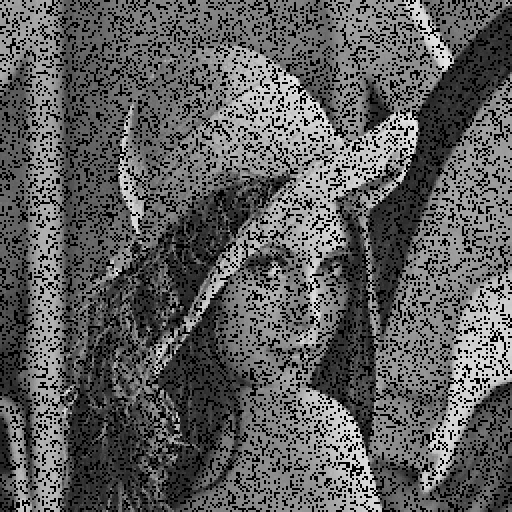
\includegraphics[width=\textwidth]{Chapter5/Images/lenna_haar1.png}
    \caption{Scale 1: PSNR = 11.75}
  \end{subfigure}
  \begin{subfigure}{0.4\textwidth}
    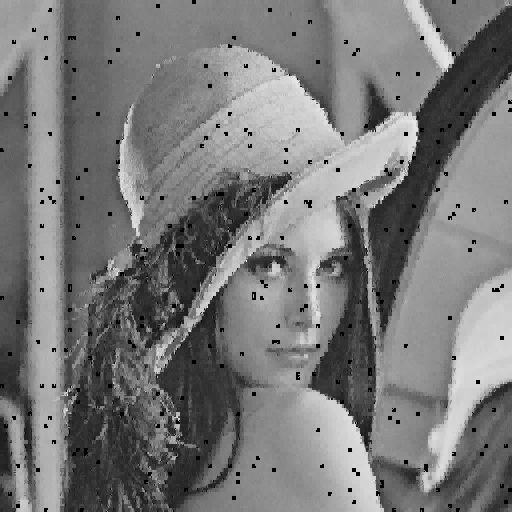
\includegraphics[width=\textwidth]{Chapter5/Images/lenna_haar2.png}
    \caption{Scale 2: PSNR = 21.78}
  \end{subfigure}
  \begin{subfigure}{0.4\textwidth}
    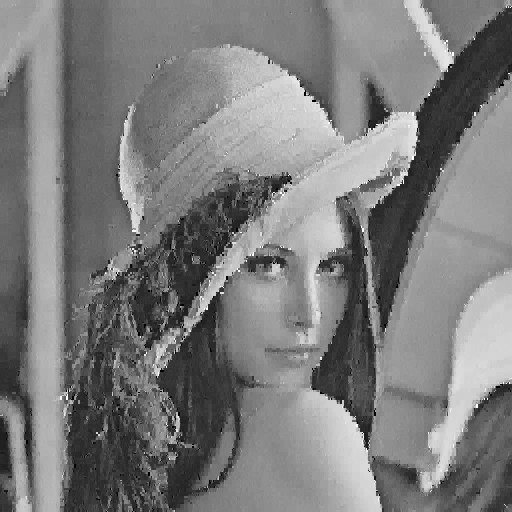
\includegraphics[width=\textwidth]{Chapter5/Images/lenna_haar3.png}
    \caption{Scale 3: PSNR = 24.15}
  \end{subfigure}
  \begin{subfigure}{0.4\textwidth}
    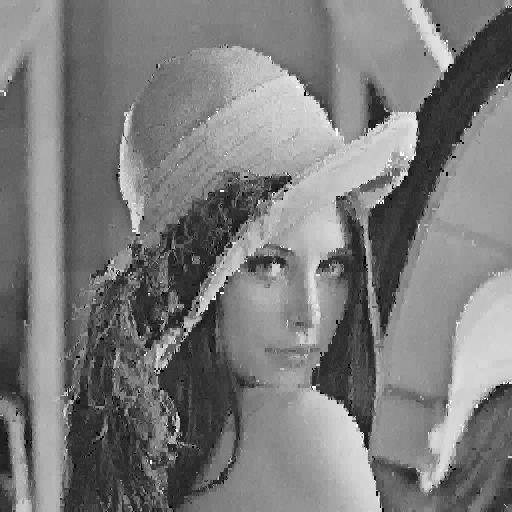
\includegraphics[width=\textwidth]{Chapter5/Images/lenna_haar4.png}
    \caption{Scale 4: PSNR = 23.72}
  \end{subfigure}  
  \caption[Reconstruction of masked image signals using Haar wavelets at various scales]{Reconstruction if the image in Figure \ref{fig:lenna_mask} using the RVM with Haar wavelets at various scales.
    We use the \emph{Peak Signal-to-Noise Ratio (PSNR)} (see Chapter \ref{ch:results}) as our performance metric. The larger the PSNR, the more accurate the reconstruction.}
  \label{fig:lenna_rvm}
\end{figure}

We see that the scale of the wavelet basis has a strong effect on the quality of the reconstruction.
Wavelets at lower scales can fail to reconstruct the entire image, but generally give a more accurate reconstruction at the portion of the image where they succeed.
On the other, wavelets at larger scales typically achieve a reconstruction of the entire image at the cost of increased blurring or pixelation.
This conflict can be seen in Figure \ref{fig:lenna_rvm} by contrasting panel (c) with panel (d):
They both achieve a reconstruction of the entire image, but scale 3 outperforms scale 4 in this example.
Moreover, if we compare panel (b) with panel (d), we see that, in the part of the image where the recovery succeeds, the scale 2 reconstruction manages to recover finer details than both scale 3 and scale 4.

To explain why this tradeoff exists, recall that two-dimensional Haar wavelets at scale $s$ have a support of size up to $2^s\times 2^s$.
Thus, at small scales, the support of the individual basis functions is small.
For example, suppose $s=1$.
In this case, each Haar basis functions covers an area of $2\times 2$ pixels (see Figure \ref{fig:haar2_basis}).
Using these wavelets, we can capture very local relationships between the pixels.
This allows us to recover finer details in the reconstruction.

However, it can also lead to the formation of black pixels.
At scale 1, each column $j$ of the Haar basis matrix $\bm \Psi$ contains exactly 4 non-zero entries corresponding to the four pixel locations that are covered by the $j$th basis function.
If the masked image happens to be missing data at all four of these locations, the corresponding rows of the basis matrix $\bm\Psi$ will be deleted when forming the design matrix $\bm\Phi=\bm\Theta\bm\Psi$.
Therefore, column $j$ of the design matrix will be zero.
The same is true for the three columns that correspond to the remaining locations that were covered by basis function $j$.

The SSBL algorithm will generally not select any columns that are completely zero, since they offer no change to the marginal likelihood.
The consequence is that the corresponding entries in the posterior mean $\bm\mu$ of $\bm w$ will remain zero.
The resulting reconstruction (\ref{eqn:bcs_recover}) will therefore be unable to recover the $2\times 2$ patch covered by basis function $j$.

This problem can be mitigated by using larger scales since, for any given total number of missing pixels, it is less likely that larger square patches of the masked image are completely void of data.
However, the SSBL Algorithm generally prefers to add basis functions with larger support to the model, since they typically cause a larger increase in the Marginal Likelihood.
The result is that we get a more blurred reconstruction and lose the finer details, even in parts of the image that would have been accurately recovered at smaller scales.





\subsection{Multi-Scale Cascade of Estimations Algorithm}
The \emph{Multi-Scale Cascade of Estimations} (MSCE) algorithm was developed by \cite{pilikos2014} to this tradeoff between inaccurate but complete reconstructions and accurate but incomplete reconstructions.

To explain the algorithm, note that, in the interpolation problem, the BCS reconstruction (\ref{eqn:bcs_recover}) is equivalent to computing the mean (\ref{rvm:pred_mean}) of the predictive distribution (\ref{rvm:predictive}) of the entire signal $\bm v$.
Moreover, we can compute the predictive variance (\ref{rvm:pred_var}) (or error-bars) for each estimate:
\begin{equation}
\label{eqn:msce_error}
  (\sigma^2)^* = \sigma^2 +\bm\psi(\bm x^*)^T\bm\Sigma\bm\psi(\bm x).
\end{equation}

The MSCE algorithm uses these error bars to construct a cascade of BCS algorithms, that builds up the scale of the Haar wavelets.

We begin by executing the BCS algorithm using Haar wavelets at the first scale.
Next, we compute equation (\ref{eqn:msce_error}) for each location in the signal in which originally had missing data.
If $(\sigma^2)^*$ is small, but larger than the noise variance $\sigma^2$, we trust the estimate and accept it. 
If $(\sigma^2)^*$ is large, we do not trust the estimate and reject it.

If $(\sigma^2)^*$ is equal to $\sigma^2$, then $\bm\psi(\bm x^*)^T\bm\Sigma\bm\psi(\bm x^*) = 0$. 
This means that $\bm\psi(\bm x^*) = 0$ since, by postive definiteness of $\bm\Sigma$, $\bm\psi(\bm x^*)^T\bm\Sigma\bm\psi(\bm x^*) > 0$ unless $\bm\psi(\bm x^*) = 0$.
Thus, the RVM predicted the pixel value at location $\bm x^*$ to be zero. 
Since the recovery of the pixel was unsuccessful in this case, we reject the estimate.

The output of the current cascade becomes the target vector of the next cascade.
The new basis matrix is constructed using Haar wavelets that are one scale higher than in the previous cascade.

This process it repeated until we no more signal values marked as missing, or until some pre-defined maximum for the scale of the Haar basis is reached.

We have summarized the MCSE in Algorithm \ref{alg3}.

\begin{algorithm}
  \caption{Multi-Scale Cascade of Estimations \cite{pilikos2014}}
  \label{alg3}
  \begin{algorithmic}[1]
    \State Set $s=1$
    \State Let $\bm y_1 = \bm y$
    \While {$s \leq s_{max}$}
    \State Form basis matrix $\bm\Psi$ using Haar wavelets at scale $s$
    \State Call Sequential Sparse Bayesian Learning Algorithm with target
    \Statex $\qquad$ vector $\bm y_j$ and design matrix $\bm\Phi=\bm\Theta\bm\Psi$ to get the estimate $\bm{\hat v}_s$
    \State Compute $(\sigma^2)^*$ for all newly reconstructed pixel values using equation (\ref{eqn:msce_error})
    \State If $(\sigma^2)^* = \sigma^2$ or $(\sigma^2)^* > \tau$, discard the corresponding estimate
    \State Set $s = s+1$
    \State Let $\bm y_s$ be $\bm{\hat v}_s$ after the discarded estimates are deleted
    \EndWhile
    \State\Return $\bm v = \bm y_s$
  \end{algorithmic}
\end{algorithm}

Note that in practice, we often choose to keep any estimate for which $(\sigma^2)^*>\sigma^2$, so that any prediction that is not zero is trusted.

\chapter{Implementation Details}
\label{ch:code}
We have implemented the MSCE Algorithm for video signals in C++.

In this chapter, we will discuss some of the design decisions and optimizations that went into the implementation.

\section{Blockwise Reconstruction}
Let $\bm v$ be a video signal consisting of $f$ frames with a width of $w$ and a height $h$.
Vectorizing $\bm v$ gives us a vector of length $hwf$.
In order to reconstruct such signals in the Bayesian Compressive Sensing framework (Chapter \ref{ch:msce}), we need to form the basis matrix $\bm\Psi$ which has dimensions $(hwf)\times (hwf)$.

Even for relatively small videos, the memory requirements for such large basis matrices can easily be in the order of terabytes.
As an example, consider the commonly used \emph{CIF (Common Intermediate Format)}.
CIF videos have a spatial resolution of $352 \times 288$.
For a CIF video containing 100 frames, the required memory for storing $\bm\Psi$ as \emph{floats} is 
\begin{equation*}
(288\times 352\times 100)^2 \times 4 \mbox{ bytes} = 4.11 \times 10^{14} \mbox{ bytes} = 411 \mbox{ TB}
\end{equation*}

In our code, we address the problem by performing a \emph{blockwise reconstruction}.
We split the input signal into small sub-blocks of size $2^{j_1}\times 2^{j_2}\times 2^{j_3}$.
A typical size of such a block is $16\times 16\times 16$ (a so-called ``macroblock'').

The blocks are sequentially passed to the MSCE algorithm and after each block has been reconstructed , we put them back together to obtained the recovered video.

Note that the size of the block restricts the number of cascades in the MSCE algorithm.
To run the algorithm up to scale $s$, we require a block size of at least $2^s\times 2^s\times 2^s$.

\section{Code Optimization}
\subsection{Parallelization}
In the blockwise reconstruction, each block is processed independently from the others.
Therefore, we have added an option to the code to process the blocks in parallel.
Using the \emph{Message Passing Interface} (MPI), we run the program on several processors, splitting the workload evenly between them. This generally leads to a very significant speedup.

However, if the blocksize is too small, the communication between processes - when gathering the results - will dominate over the actual computation time.
Initial tests seem to indicate that, in order to achieve a significant increase in the execution time, the blocks should be at least of size $4\times4\times4$ before switching to parallel mode.


\subsection{Fixed Noise Variance}
At each stage of the MSCE algorithm, we keep the noise variance $\sigma^2$ fixed, while training the Sparse Bayesian Learning model.
As noted in Section \ref{sect:ssbl}, doing so allows us to use the efficient update formulae in \cite{tipping2003} which speed up training.

\subsection{Modified RVM Training}
In the MSCE, the RVM is trained using Algorithm \ref{rvm:alg2}.
We use a slightly modified version of the training algorithm in which we only consider addition of basis functions to the model.

At each iteration, we add the basis vector $\bm\phi$ that results in the largest increase of the marginal likelihood.
We continue to do so until none of the remaining candidate basis functions cause an increase in log marginal likelihood that is above the convergence threshold.

For the problem of image and video reconstruction, this modified algorithm gives qualitatively similar results to the unmodified version \cite{pilikos2014}. However, it can lead to a significant reduction in the runtime of the algorithm.



\chapter{Simulations}
\label{ch:results}

\section{Performance Metrics}
In this section, we will introduce three performance metrics that are often used to measure the quality of reconstructed images and videos.

Let $\bm{\hat v} \in\mathbb{R}^M$ be a reconstructed signal (in vectorized form) and let $\bm v$ be the corresponding orginal signal.
The \emph{mean square error} (MSE) of the reconstruction is defined as
\begin{equation*}
  \mse(\bm{\hat v}) = \frac{\sum_{i=1}^M (\hat v_i - v_i)^2}{M}
\end{equation*}
The MSE is zero if and only if we $\bm{\hat v}$ is an exact reconstruction of $\bm v$.

Using the MSE, we can compute the \emph{Peak Signal-to-Noise Ratio} (PSNR) of the reconstruction:
\begin{equation*}
  \psnr(\bm{\hat v}) = 10 \cdot \log_{10} \left(\frac{R^2}{\mse(\bm{\hat v})}\right)
\end{equation*}
where $R$ is the maximum fluctuation in the input signal data type. 
For grayscale images or videos in which the pixel values are stored as 8-bit unsigned integers, we have that $R = 256$.

The PSNR is usually expressed in term of decibel (dB). 
Higher values of the PSNR correspond to more accurate reconstructions.
The PSNR is widely used in the image and video compression literature to measure the quality of a compressed signal.
Generally, when comparing the reconstruction quality, the PSNR should only be used if it was measured on the same signal.

The final performance metric that we compute is the \emph{relative reconstruction error}.
It is given by
\begin{equation*}
  \rre(\bm{\hat v}) = \frac{||\bm{\hat v} - \bm v||_2}{||\bm v||_2}
\end{equation*}
This is the metric that was used in \cite{ji2008} and \cite{pilikos2014}.

\section{Experiments}
In this section, we perform experiments in order to get an idea of how the different components of the implementation perform.
All simulations were run on the ``foreman'' test video using blocks of size $8\times 8\times 8$.

\subsection{MSCE vs BCS}
We compare the performance of using cascades over individual BCS

\subsection{DCT vs Haar(3)}
In Figure \ref{fig:sim_basis}, we compareshows a comparison between using the DCT basis and the Haar basis.

\subsection{Gaussan vs Bernoulli vs Mask}
We compare 

\subsection{Haar Scales with Gaussian \texorpdfstring{$\bm\Theta$}{[Theta]}}

%% CASCADE
\begin{figure}
  \centering
  \begin{tikzpicture}[scale = 0.8,baseline]
    \begin{axis}[
      xlabel=$N/M$ (\%),
      ylabel=$\rre$ (\%),
      xmin=0, xmax = 100,
      ymin = 0, ymax = 0.2,
      scaled ticks=false,
      yticklabel style={
        /pgf/number format/precision=2,
        /pgf/number format/fixed,
      }
      ]
      \addplot table [x=pc, y=rre] {Chapter7/Images/MSCE.dat};      
      \addlegendentry{MSCE}
      \addplot table [x=pc, y=rre] {Chapter7/Images/MASK_3.dat};      
      \addlegendentry{BCS Scale 3}
      \addplot table [x=pc, y=rre] {Chapter7/Images/MASK_2.dat};     
      \addlegendentry{BCS Scale 2}
      \addplot table [x=pc, y=rre] {Chapter7/Images/MASK_1.dat};
      \addlegendentry{BCS Scale 1}
    \end{axis}
  \end{tikzpicture}
  % 
  \hskip 10pt
  % 
  \begin{tikzpicture}[scale = 0.8,baseline]
    \begin{axis}[
      xlabel=$N/M$ (\%),
      ylabel=$\psnr$ (dB),
      xmin=0, xmax = 90, 
      scaled ticks=false,
      legend style={
        at={(0.03,1.04)},
        anchor=north west,
      },
      yticklabel style={
        /pgf/number format/precision=2,
        /pgf/number format/fixed,
      }
      ]
      \addplot table [x=pc, y=psnr] {Chapter7/Images/MSCE.dat};      
      \addlegendentry{MSCE}
      \addplot table [x=pc, y=psnr] {Chapter7/Images/MASK_3.dat};
      \addlegendentry{BCS Scale 3}
      \addplot table [x=pc, y=psnr] {Chapter7/Images/MASK_2.dat};
      \addlegendentry{BCS Scale 2}
      \addplot table [x=pc, y=psnr] {Chapter7/Images/MASK_1.dat};
      \addlegendentry{BCS Scale 1}
    \end{axis}
  \end{tikzpicture}
\caption{Performance of MSCE with 3 cascades and uniform Masks}
\label{fig:sim_msce}
\end{figure}

%% BASIS
\begin{figure}
  \centering
  \begin{tikzpicture}[scale = 0.8,baseline]
    \begin{axis}[
      xlabel=$N/M$ (\%),
      ylabel=$\rre$ (\%),
      xmin=0, xmax = 100,
      ymin = 0, 
      scaled ticks=false,
      yticklabel style={
        /pgf/number format/precision=2,
        /pgf/number format/fixed,
      }
      ]
      \addplot table [x=pc, y=rre] {Chapter7/Images/GAUSS_DCT.dat};      
      \addlegendentry{DCT}
      \addplot table [x=pc, y=rre] {Chapter7/Images/GAUSS_HAAR.dat};      
      \addlegendentry{Haar}
    \end{axis}
  \end{tikzpicture}
  % 
  \hskip 10pt
  % 
  \begin{tikzpicture}[scale = 0.8,baseline]
    \begin{axis}[
      xlabel=$N/M$ (\%),
      ylabel=$\psnr$ (dB),
      xmin=0, xmax = 90,      
      scaled ticks=false,
      legend style={
        at={(0.03,0.98)},
        anchor=north west,
      },
      yticklabel style={
        /pgf/number format/precision=2,
        /pgf/number format/fixed,
      }
      ]
      \addplot table [x=pc, y=psnr] {Chapter7/Images/GAUSS_DCT.dat};      
      \addlegendentry{DCT}
      \addplot table [x=pc, y=psnr] {Chapter7/Images/GAUSS_HAAR.dat};      
      \addlegendentry{Haar}
    \end{axis}
  \end{tikzpicture}
\caption{DCT vs Haar DWT (scale 3) with Gaussian measurements}
\label{fig:sim_basis}
\end{figure}

%% SENSORS
\begin{figure}
  \centering
  \begin{tikzpicture}[scale = 0.8,baseline]
    \begin{axis}[
      xlabel=$N/M$ (\%),
      ylabel=$\rre$ (\%),
      xmin=0, xmax = 100,
      ymin = 0, 
      scaled ticks=false,
      yticklabel style={
        /pgf/number format/precision=2,
        /pgf/number format/fixed,
      }
      ]
      \addplot table [x=pc, y=rre] {Chapter7/Images/GAUSS_DCT.dat};      
      \addlegendentry{Gauss}
      \addplot table [x=pc, y=rre] {Chapter7/Images/BERN_DCT.dat};      
      \addlegendentry{Bernoulli}
      \addplot table [x=pc, y=rre] {Chapter7/Images/MASK_DCT.dat};      
      \addlegendentry{Mask}
    \end{axis}
  \end{tikzpicture}
  % 
  \hskip 10pt
  % 
  \begin{tikzpicture}[scale = 0.8,baseline]
    \begin{axis}[
      xlabel=$N/M$ (\%),
      ylabel=$\psnr$ (dB),
      xmin=0, xmax = 90,      
      scaled ticks=false,
      legend style={
        at={(0.03,0.98)},
        anchor=north west,
      },
      yticklabel style={
        /pgf/number format/precision=2,
        /pgf/number format/fixed,
      }
      ]
      \addplot table [x=pc, y=psnr] {Chapter7/Images/GAUSS_DCT.dat};      
      \addlegendentry{Gauss}
      \addplot table [x=pc, y=psnr] {Chapter7/Images/BERN_DCT.dat};      
      \addlegendentry{Bernoulli}
      \addplot table [x=pc, y=psnr] {Chapter7/Images/MASK_DCT.dat};      
      \addlegendentry{Mask}
    \end{axis}
  \end{tikzpicture}
\caption{Gaussian vs Bernoulli vs Mask (uniform) with DCT basis}
\label{fig:sim_sensor}
\end{figure}

%% SCALES
\begin{figure}
  \centering
  \begin{tikzpicture}[scale = 0.8,baseline]
    \begin{axis}[
      xlabel=$N/M$ (\%),
      ylabel=$\rre$ (\%),
      xmin=0, xmax = 100,
      ymin = 0, 
      scaled ticks=false,
      yticklabel style={
        /pgf/number format/precision=2,
        /pgf/number format/fixed,
      }
      ]
      \addplot table [x=pc, y=rre] {Chapter7/Images/HAAR_GAUSS_1.dat};      
      \addlegendentry{Scale 1}
      \addplot table [x=pc, y=rre] {Chapter7/Images/HAAR_GAUSS_2.dat};
      \addlegendentry{Scale 2}
      \addplot table [x=pc, y=rre] {Chapter7/Images/HAAR_GAUSS_3.dat};
      \addlegendentry{Scale 3}
    \end{axis}
  \end{tikzpicture}
  % 
  \hskip 10pt
  % 
  \begin{tikzpicture}[scale = 0.8,baseline]
    \begin{axis}[
      xlabel=$N/M$ (\%),
      ylabel=$\psnr$ (dB),
      xmin=0, xmax = 90,      
      scaled ticks=false,
      legend style={
        at={(0.03,0.98)},
        anchor=north west,
      },
      yticklabel style={
        /pgf/number format/precision=2,
        /pgf/number format/fixed,
      }
      ]
      \addplot table [x=pc, y=psnr] {Chapter7/Images/HAAR_GAUSS_1.dat};
      \addlegendentry{Scale 1}
      \addplot table [x=pc, y=psnr] {Chapter7/Images/HAAR_GAUSS_2.dat};
      \addlegendentry{Scale 2}
      \addplot table [x=pc, y=psnr] {Chapter7/Images/HAAR_GAUSS_3.dat};
      \addlegendentry{Scale 3}
    \end{axis}
  \end{tikzpicture}
\caption{Haar wavelets at different scales with Gaussian measurements (fixed block size)}
\label{fig:sim_scales}
\end{figure}

\clearpage

\section{Example Results}

\begin{figure}[!ht]
  \centering
  \textbf{\hspace{0.2in} Frame 2 \hspace{1.5in} Frame 19\hspace{0.5in}\vspace{0.2in}}
  \begin{subfigure}{0.4\textwidth}
    \centering
    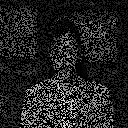
\includegraphics[width=0.8\textwidth]{Chapter7/Images/akiyo40_masked_2.png}
    \caption{Corrupted}
  \end{subfigure}
  \begin{subfigure}{0.4\textwidth}
    \centering
    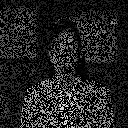
\includegraphics[width=0.8\textwidth]{Chapter7/Images/akiyo40_masked_19.png}
    \caption{Corrupted}
  \end{subfigure}
  \begin{subfigure}{0.4\textwidth}
    \centering
    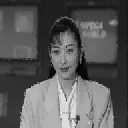
\includegraphics[width=0.8\textwidth]{Chapter7/Images/akiyo40_rec_2.png}
    \caption{Recovered}
  \end{subfigure}
  \begin{subfigure}{0.4\textwidth}
    \centering
    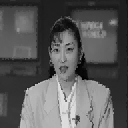
\includegraphics[width=0.8\textwidth]{Chapter7/Images/akiyo40_rec_19.png}
    \caption{Recovered}
  \end{subfigure}
  \begin{subfigure}{0.4\textwidth}
    \centering
    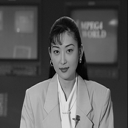
\includegraphics[width=0.8\textwidth]{Chapter7/Images/akiyo40_orig_2.png}
    \caption{Original}
  \end{subfigure}
  \begin{subfigure}{0.4\textwidth}
    \centering
    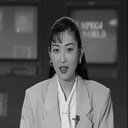
\includegraphics[width=0.8\textwidth]{Chapter7/Images/akiyo40_orig_19.png}
    \caption{Original}
  \end{subfigure}
  \caption{Reconstruction of $128\times 128\times 128$ video signal ``akiyo'' from 40\% of the measurement using the MSCE with 3 cascades. Mask decimation pattern is uniform. $\psnr = 30.02$}
\end{figure}

\begin{figure}
  \centering
  \textbf{\hspace{0.2in} Frame 32 \hspace{1.5in} Frame 52\hspace{0.5in}\vspace{0.1in}}
  \begin{subfigure}{0.4\textwidth}
    \centering
    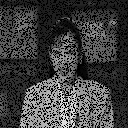
\includegraphics[width=0.9\textwidth]{Chapter7/Images/akiyo70_masked_32.png}
    \caption{Corrupted}
  \end{subfigure}
  \begin{subfigure}{0.4\textwidth}
    \centering
    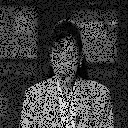
\includegraphics[width=0.9\textwidth]{Chapter7/Images/akiyo70_masked_52.png}
    \caption{Corrupted}
  \end{subfigure}
  \begin{subfigure}{0.4\textwidth}
    \centering
    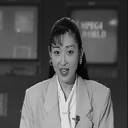
\includegraphics[width=.9\textwidth]{Chapter7/Images/akiyo70_rec_32.png}
    \caption{Recovered}
  \end{subfigure}
  \begin{subfigure}{0.4\textwidth}
    \centering
    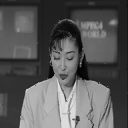
\includegraphics[width=.9\textwidth]{Chapter7/Images/akiyo70_rec_52.png}
    \caption{Recovered}
  \end{subfigure}
  \begin{subfigure}{0.4\textwidth}
    \centering
    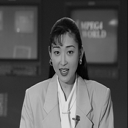
\includegraphics[width=.9\textwidth]{Chapter7/Images/akiyo70_orig_32.png}
    \caption{Original}
  \end{subfigure}
  \begin{subfigure}{0.4\textwidth}
    \centering
    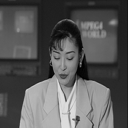
\includegraphics[width=.9\textwidth]{Chapter7/Images/akiyo70_orig_52.png}
    \caption{Original}
  \end{subfigure}
  \caption{Reconstruction of $128\times 128\times 128$ video signal ``akiyo'' from 70\% of the measurement using the MSCE with 3 cascades. Mask decimation pattern is uniform. $\psnr = 36.86$}
\end{figure}

\begin{figure}
  \centering
  \textbf{\hspace{0.2in} Frame 18 \hspace{1.5in} Frame 22\hspace{0.5in}\vspace{0.1in}}
  \begin{subfigure}{0.4\textwidth}
    \centering
    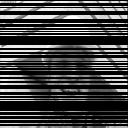
\includegraphics[width=.9\textwidth]{Chapter7/Images/foreman40_masked_18.png}
    \caption{Corrupted}
  \end{subfigure}
  \begin{subfigure}{0.4\textwidth}
    \centering
    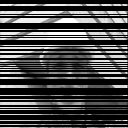
\includegraphics[width=.9\textwidth]{Chapter7/Images/foreman40_masked_22.png}
    \caption{Corrupted}
  \end{subfigure}
  \begin{subfigure}{0.4\textwidth}
    \centering
    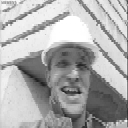
\includegraphics[width=.9\textwidth]{Chapter7/Images/foreman40_rec_18.png}
    \caption{Recovered}
  \end{subfigure}
  \begin{subfigure}{0.4\textwidth}
    \centering
    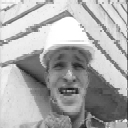
\includegraphics[width=.9\textwidth]{Chapter7/Images/foreman40_rec_22.png}
    \caption{Recovered}
  \end{subfigure}
  \begin{subfigure}{0.4\textwidth}
    \centering
    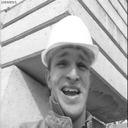
\includegraphics[width=.9\textwidth]{Chapter7/Images/foreman40_orig_18.png}
    \caption{Original}
  \end{subfigure}
  \begin{subfigure}{0.4\textwidth}
    \centering
    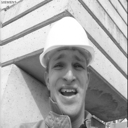
\includegraphics[width=.9\textwidth]{Chapter7/Images/foreman40_orig_22.png}
    \caption{Original}
  \end{subfigure}
  \caption{Reconstruction of $128\times 128\times 128$ video signal ``foreman'' from 40\% of the measurement using the MSCE with 3 cascades. Mask decimation pattern is: horizontal lines that are randomly generated for each frame. $\psnr = 25.50$}
\end{figure}


\begin{figure}
  \centering
  \textbf{\hspace{0.2in} Frame 18 \hspace{1.5in} Frame 22\hspace{0.5in}\vspace{0.1in}}
  \begin{subfigure}{0.4\textwidth}
    \centering
    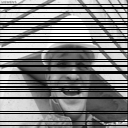
\includegraphics[width=.9\textwidth]{Chapter7/Images/foreman70_masked_18.png}
    \caption{Corrupted}
  \end{subfigure}
  \begin{subfigure}{0.4\textwidth}
    \centering
    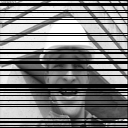
\includegraphics[width=.9\textwidth]{Chapter7/Images/foreman70_masked_22.png}
    \caption{Corrupted}
  \end{subfigure}
  \begin{subfigure}{0.4\textwidth}
    \centering
    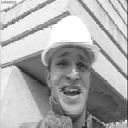
\includegraphics[width=.9\textwidth]{Chapter7/Images/foreman70_rec_18.png}
    \caption{Recovered}
  \end{subfigure}
  \begin{subfigure}{0.4\textwidth}
    \centering
    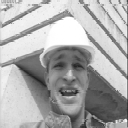
\includegraphics[width=.9\textwidth]{Chapter7/Images/foreman70_rec_22.png}
    \caption{Recovered}
  \end{subfigure}
  \begin{subfigure}{0.4\textwidth}
    \centering
    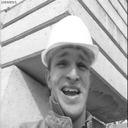
\includegraphics[width=.9\textwidth]{Chapter7/Images/foreman70_orig_18.png}
    \caption{Original}
  \end{subfigure}
  \begin{subfigure}{0.4\textwidth}
    \centering
    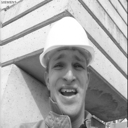
\includegraphics[width=.9\textwidth]{Chapter7/Images/foreman70_orig_22.png}
    \caption{Original}
  \end{subfigure}
  \caption{Reconstruction of $128\times 128\times 128$ video signal ``foreman'' from 70\% of the measurement using the MSCE with 3 cascades. Mask decimation pattern is: horizontal lines that are randomly generated for each frame. $\psnr = 30.32$}
\end{figure}

\begin{figure}
  \centering
  \textbf{\hspace{0.2in} Frame 11 \hspace{1.5in} Frame 12\hspace{0.5in}\vspace{0.1in}}
  \begin{subfigure}{0.4\textwidth}
    \centering
    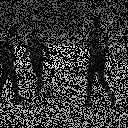
\includegraphics[width=.9\textwidth]{Chapter7/Images/soccer40_masked_11.png}
    \caption{Corrupted}
  \end{subfigure}
  \begin{subfigure}{0.4\textwidth}
    \centering
    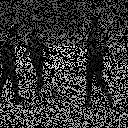
\includegraphics[width=.9\textwidth]{Chapter7/Images/soccer40_masked_12.png}
    \caption{Corrupted}
  \end{subfigure}
  \begin{subfigure}{0.4\textwidth}
    \centering
    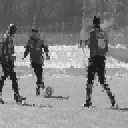
\includegraphics[width=.9\textwidth]{Chapter7/Images/soccer40_rec_11.png}
    \caption{Recovered}
  \end{subfigure}
  \begin{subfigure}{0.4\textwidth}
    \centering
    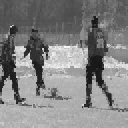
\includegraphics[width=.9\textwidth]{Chapter7/Images/soccer40_rec_12.png}
    \caption{Recovered}
  \end{subfigure}
  \begin{subfigure}{0.4\textwidth}
    \centering
    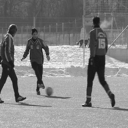
\includegraphics[width=.9\textwidth]{Chapter7/Images/soccer40_orig_11.png}
    \caption{Original}
  \end{subfigure}
  \begin{subfigure}{0.4\textwidth}
    \centering
    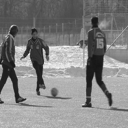
\includegraphics[width=.9\textwidth]{Chapter7/Images/soccer40_orig_12.png}
    \caption{Original}
  \end{subfigure}
  \caption{Reconstruction of $128\times 128\times 128$ video signal ``soccer'' from 40\% of the measurement using the MSCE with 3 cascades. Mask decimation pattern is: missing pixels that are constant across the frames. $\psnr = 24.84$}
\end{figure}



\begin{figure}
  \centering
  \textbf{\hspace{0.2in} Frame 11 \hspace{1.5in} Frame 12\hspace{0.5in}\vspace{0.1in}}
  \begin{subfigure}{0.4\textwidth}
    \centering
    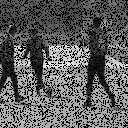
\includegraphics[width=.9\textwidth]{Chapter7/Images/soccer70_masked_11.png}
    \caption{Corrupted}
  \end{subfigure}
  \begin{subfigure}{0.4\textwidth}
    \centering
    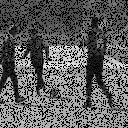
\includegraphics[width=.9\textwidth]{Chapter7/Images/soccer70_masked_12.png}
    \caption{Corrupted}
  \end{subfigure}
  \begin{subfigure}{0.4\textwidth}
    \centering
    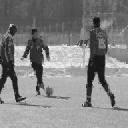
\includegraphics[width=.9\textwidth]{Chapter7/Images/soccer70_rec_11.png}
    \caption{Recovered}
  \end{subfigure}
  \begin{subfigure}{0.4\textwidth}
    \centering
    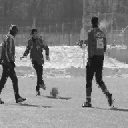
\includegraphics[width=.9\textwidth]{Chapter7/Images/soccer70_rec_12.png}
    \caption{Recovered}
  \end{subfigure}
  \begin{subfigure}{0.4\textwidth}
    \centering
    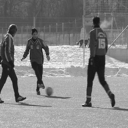
\includegraphics[width=.9\textwidth]{Chapter7/Images/soccer70_orig_11.png}
    \caption{Original}
  \end{subfigure}
  \begin{subfigure}{0.4\textwidth}
    \centering
    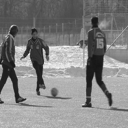
\includegraphics[width=.9\textwidth]{Chapter7/Images/soccer70_orig_12.png}
    \caption{Original}
  \end{subfigure}
  \caption{Reconstruction of $128\times 128\times 128$ video signal ``soccer'' from 70\% of the measurement using the MSCE with 3 cascades. Mask decimation pattern is: missing pixels that are constant across the frames. $\psnr = 29.35$}
\end{figure}

\begin{figure}
  \centering
  \textbf{\hspace{0.5in} Frame 21 \hspace{1.5in} Frame 151\hspace{0.5in}\vspace{0.2in}}
  \begin{subfigure}{0.4\textwidth}
    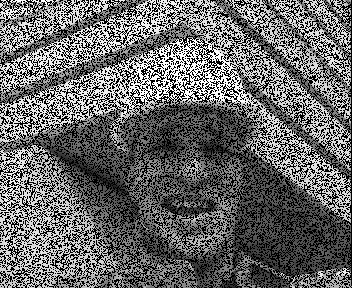
\includegraphics[width=\textwidth]{Chapter5/Images/foreman_masked_21.png}
    \caption{Corrupted}
  \end{subfigure}
  \begin{subfigure}{0.4\textwidth}
    \includegraphics[width=\textwidth]{Chapter5/Images/foreman_masked_151.png}
    \caption{Corrupted}
  \end{subfigure}
  \begin{subfigure}{0.4\textwidth}
    \includegraphics[width=\textwidth]{Chapter5/Images/foreman_rec_21.png}
    \caption{Recovered}
  \end{subfigure}
  \begin{subfigure}{0.4\textwidth}
    \includegraphics[width=\textwidth]{Chapter5/Images/foreman_rec_151.png}
    \caption{Recovered}
  \end{subfigure}
  \begin{subfigure}{0.4\textwidth}
    \includegraphics[width=\textwidth]{Chapter5/Images/foreman_orig_21.png}
    \caption{Original}
  \end{subfigure}
  \begin{subfigure}{0.4\textwidth}
    \includegraphics[width=\textwidth]{Chapter5/Images/foreman_orig_151.png}
    \caption{Original}
  \end{subfigure}
  \caption[Example output of our video interpolator]{Example of a masked video signal, where only 60\% of the pixel values are known (a-b). 
    Reconstruction via the MSCE Algorithm using 2 cascades (PSNR: 28.6) (c-d).
    Original video (e-f).}
  \label{fig:foreman_masked}
\end{figure}


\chapter{Conclusion}
\label{ch:conclusion}

For the MPhil thesis, we set out to develop a generic Compressive Sensing algorithm that provides high quality reconstructions of video signals from relatively small numbers of samples.


In this thesis, we investigated the efficacy of the Bayesian Compressive Sensing framework for efficient reconstruction of highly under-sampled video signals.
We developed an extension to the Multi-Scale Cascade of Estimations algorithm that achieves near-perfect reconstructions of videos from a very small set of measurements.

To do so, we constructed three-dimensional wavelet basis functions that allow for a highly compressible representation of the video signal.
Compressive Sensing inversion is then formulated as a machine learning problem and the Relevance Vector Machine was employed to find highly sparse solutions.
To boost performance, a cascade of RVMs it built that exploits the multi-resolution properties of wavelet basis functions.

In order to deal with the large memory requirements of the algorithm, the reconstruction is performed in blockwise fashion.
We have also implemented the method as a distributed program, resulting in dramatically reduced execution times.

Future research could improve performance by extending these methods in various ways.
In order to fully harness the power of the MSCE for video interpolation, the implentation should be extended to accommodate different kinds of wavelets.
Using the simple Haar wavelets, the MSCE struggles to outperform a BCT that uses DCT basis functions.
It only shows its advantage in extremely undersampled situations ($N < 0.2M$).
Alternative sets of waveles, such as the CDF-9/7 wavelet that is used by the JPEG2000 format, may lead to sparser representations of the video signals. 

Furthermore, the speed of the algorithm can be increased by using a multi-threaded implementation of the Sequential Sparse Bayesian Learning Algorithm. 

Development of Bayesian approaches to Compressive Sensing systems is an active area of research.




%\setboolean{@twoside}{false}
%\includepdf[pages={1},angle=270]{gantt.pdf}
%\section*{Acknowledgements}
%Here I acknowledge the assistance of my supervisor, my industrial sponsor,
%and the effects of caffeine on my ability to produce this report on time.

%% The Appendices part is started with the command \appendix;
%% appendix sections are then done as normal sections
%\appendix

%% References
%%
%% Following citation commands can be used in the body text:
%% Usage of \cite is as follows:
%%   \cite{key}         ==>>  [#]
%%   \cite[chap. 2]{key} ==>> [#, chap. 2]
%%

%% References with bibTeX database:
%\section*{Bibliography}
\bibliographystyle{elsarticle-num}
%\bibliographystyle{apa}
\bibliography{referencesRVM.bib}

%% Authors are advised to submit their bibtex database files. They are
%% requested to list a bibtex style file in the manuscript if they do
%% not want to use elsarticle-num.bst.

%% References without bibTeX database:

% \begin{thebibliography}{00}

%% \bibitem must have the following form:
%%   \bibitem{key}...
%%

% \bibitem{}

% \end{thebibliography}


\end{document}

%%
%% End of file `rvm.tex'.